\chapter{Contour Integration}
\label{sec:contour}
\chaptermark{Contour integration}

There is increasing evidence that visual processing of objects makes use of both feedforward and feedback streams of information. However, it is unclear how higher visual areas know which features belong to an object and what feedback signals to send back. Here, we develop a recurrent neural model to address these questions in the context of contour integration and figure-ground segregation. A key feature of our model is the use of grouping neurons whose activity represents tentative objects based on the integration of local feature information. Grouping neurons send excitatory feedback to the same local feature neurons that caused their activation, while inhibition
at both the local feature level and the object representation level help to select between competing interpretations of the visual scene.
Our model is able to explain several sets of neurophysiological results~\citep{Zhou_etal00,Qiu_etal07,Chen_etal14}, and makes
testable predictions about the influence of feedback and attention on
neural responses across different visual areas. Our model also provides a framework for understanding how object-based attention is able to select both objects and the features associated with them.

\section{Introduction}
\label{intro}
Gestalt psychologists recognized the importance of the whole in influencing perception of the parts when they laid out several principles (``Gestalt laws'')for perceptual organization~\citep{Wertheimer23,Koffka35}. Contour integration, the linking of line segments into contours, and figure-ground segregation, the segmenting of objects from background, are fundamental components of perceptual organization. Both processes require combining local, low-level and global, high-level information across different visual areas in order to segment the visual scene. The interaction between feedforward and feedback streams carrying this information, as well as the contribution of top-down influences such as attention, are not well understood.

The contour integration process seems to begin in primary visual cortex (V1), where the responses of orientation selective neurons can be enhanced by placing collinear stimuli outside the receptive fields (RFs) of these neurons~\citep{Stemmler_etal95a,Polat_etal98}. Contextual interactions between V1 neurons have often been summarized using a ``local association field,'' where collinear contour elements excite each other and noncollinear elements inhibit each other \citep{Ullman92, Field_etal93}. Results from neuroanatomy lend support to these ideas, as the lateral connections within V1 predominantly link together similar-orientation cortical columns \citep{Gilbert_Wiesel89,Bosking_etal97,
  Stettler_etal02}. Computational models based on these types of
local interactions have successfully simulated the ability of V1
neurons to extract contours from complex backgrounds~\citep{Li98,Yen_Finkel98,Piech_etal13}. 

Segmenting an image into regions corresponding to objects not only requires knowledge about object contours, but also whether these contours belong to the foreground or the background. Border ownership cells that have been found in early visual areas, predominantly in secondary visual cortex (V2), appear to be dedicated to this task. Border ownership cells encode where an object is located relative to their RFs~\citep{Zhou_etal00}. When an edge of the preferred orientation is presented in its RF, a border ownership cell will respond differently depending on the side of the figure to which the edge belongs. For example, a vertical edge can belong either to an object on the left or on the right. Even though the stimuli within its RF is kept constant, a border ownership cell will respond more strongly if the edge belongs to a figure on its preferred side than its nonpreferred side. Border ownership coding has been studied using a wide variety of artificial stimuli, including those defined by luminance~\citep{Zhou_etal00}, motion~\citep{vonderHeydt_etal03a}, disparity~\citep{Qiu_vonderHeydt05}, transparency~\citep{Qiu_vonderHeydt07}, and more recently, natural stimuli~\citep{Williford_vonderHeydt14}.
% add recent Doris Tsao reference here too

To explain this phenomenon, some computational models propose to group object features by a diffusion-like process that propagates neural activity along long-range horizontal connections within early visual areas \citep{Grossberg94, Sajda_Finkel95, Zhaoping05}. However, these models have difficulties explaining the fast establishment of border ownership which appears about 25ms after the first stimulus response \citep{Zhou_etal00}. Propagation along horizontal fibers over the distances used in the experiments would imply a delay of at least $\approx 70$ms \citep[][calculations based on the conduction velocity of horizontal fibers in primate V1 cortex, we are not aware of corresponding data for V2]{Girard_etal01}. Furthermore, such models are difficult to reconcile with the observation that the time course of border ownership coding is largely independent of figure size~\citep{Sugihara_etal11}.

An alternative computational model involves populations of ``grouping cells'' which explicitly represent (in their firing rates) the perceptual organization of the visual scene ~\citep{Craft_etal07}.  These cells are reciprocally connected to border ownership (B) neurons
through feedforward and feedback connections. In an attention-to-objects task, attention targets grouping neurons, rather
than low-level features within a spatially-defined area. Therefore
attention is directed to objects, resulting in the modulation of B cell activity through feedback from grouping cells \citep{Mihalas_etal11b}.  This object-based approach is consistent with psychophysical and
neurophysiological studies \citep[\eg][]{Duncan84,Egly_etal94,Scholl01,Kimchi_etal07,Qiu_etal07,Ho_Yeh09,Poort_etal12}.

Previous experimental studies have suggested the involvement of different visual areas in contour integration and figure-ground segregation~\citep{Poort_etal12,Chen_etal14}. However, many computational models do not address how top-down influences arising from the complex interplay between different visual areas are needed to accomplish these two tasks. Here we extend previous models of perceptual organization~\citep{Craft_etal07,Mihalas_etal11b} to explain how feedback grouping circuitry can implement the mechanisms necessary to accomplish these tasks. Our model also allows us to explain
effects of object-based attention and the role of feedback in parsing visual scenes.

\begin{figure*}
\begin{center}
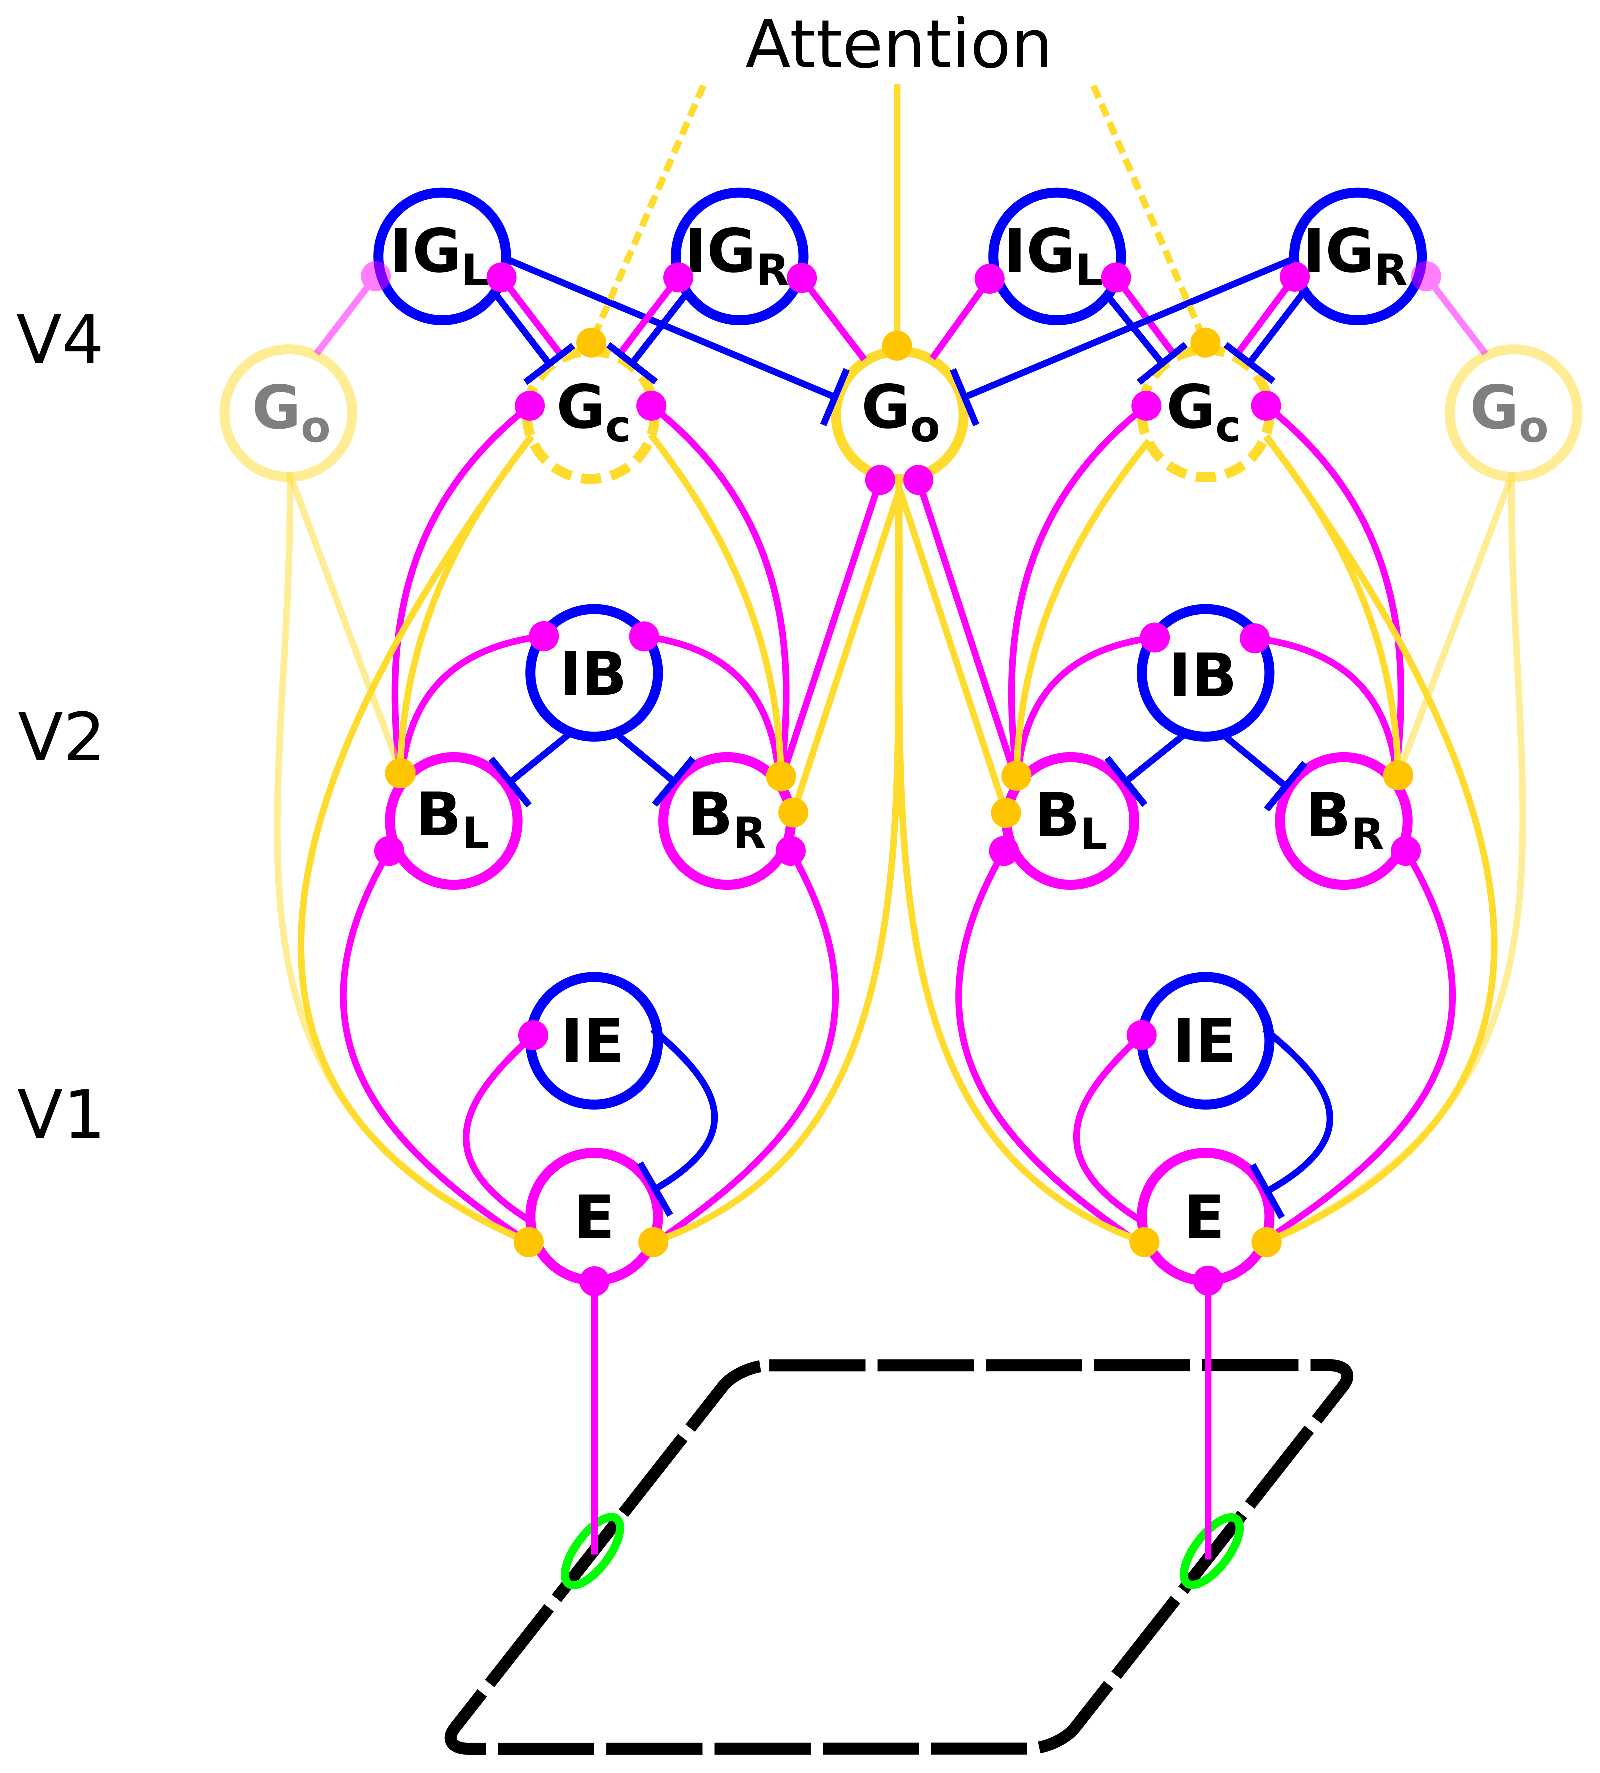
\includegraphics[width=0.5\textwidth]{Fig1.eps}
\end{center}
\caption{Structure of the model network. Each circle stands for a
  population of neurons with similar receptive fields
  and response properties. 
  Magenta, 
  blue, and orange lines represent
  feedforward excitatory, lateral inhibitory, and feedback excitatory
  projections, respectively. Edges and other local features of a figure (black dashed
  parallelogram) activate edge cells (E), whose receptive fields are
  shown by green ellipses. Edge cells project to border ownership
  cells (B) that have the same preferred orientation and 
  retinotopic position as the E cells they receive input from. However, for
  each location and preferred orientation there are two B cell
  populations with opposite side-of-figure preferences, in the example
  shown $B_{L}$ whose neurons respond preferentially when the foreground object is to the left of their receptive fields and $B_{R}$ whose members prefer the foreground to the right side of their receptive fields.\
  E cells also excite other E cells with the same preferred
  orientation (connections not shown),
  as well as a class of inhibitory cells (IE) which, in turn, inhibit
  E cells of all preferred orientations at a given location
  (only E cells of one preferred orientation are shown).
  B cells have reciprocal, forward excitatory and feedback modulatory
  connections with two types of grouping cells, $\rm G_c$ and $\rm G_o$, which integrate global context information about contours and objects,
  respectively. E cells also receive positive modulatory feedback
  from these same grouping cells. Opposing border ownership cells compete
  directly {\em via} IB cells and indirectly {\em via} grouping cells,
  which bias their activity and thus generate the response differences of
  opposing border ownership selective neurons. 
  G cell populations also directly excite
  inhibitory grouping cells (IG; again with the indices L and R),
  which inhibit $\rm G_c$ cells nonspecifically and $\rm G_o$ cells in
  all orientations except the preferred one. Top-down attention is
  modeled as input to the grouping cells and can therefore either be directed towards objects (solid lines) or contours (dashed lines) in the visual field
  (top).}
\label{Fig:anatomy}
\end{figure*}

\comment{
\section{Materials and methods} 
\label{sec:model}
\subsection{Model Structure}

%bh this is adapted from Poort et al., 2012 which used a similar model structure to explain filling-in of texture-defined figures
% This is a much simpler methods section, just to give some idea of how the model works (one reviewer did not seem to understand it), and assumes we can throw all the details not needed for understanding into a supplement/appendix section.
%
The model consists of areas V1, V2, and V4 (Figure~\ref{Fig:anatomy}). The input into the model was a binary orientation map with four orientations ($0, \pi/4, \pi/2,$ and  $3\pi/4$ relative to the horizontal). The input signal is first represented in V1 and was then propagated to V2 and V4 by feedforward connections. In addition to the feedforward projections, V4 also provides feedback to lower areas (see Supplemental Information/Appendix for equations). Neurons in higher areas have larger RFs and represent the image at a coarser resolution. RF sizes in area V4 are four times larger than the RF sizes in V2, which, in turn, are twice as large as the sizes in V1.

To achieve contour integration, we implemented excitatory lateral connections between edge (E) cells in V1 with the same orientation preference. These connections are similar to the local association fields used in other models~\citep{Li98,Piech_etal13}. Background suppression is carried out through a separate population of inhibitory (IE) cells. The input from V1 activates populations of border ownership (B) cells in V2 with opposing side-of-figure preferences. A combination of lateral connections within V2 and feedback connections from V4 (described below) are used to generate border ownership selectivity. Inhibitory (IB) cells in V2 cause inhibition between competing B cells. In V4, two different types of grouping cells exist. Contour grouping cells ($\rm G_c$) integrate local edge information and are selective for oriented contours (Figure~\ref{Fig:BG_projections}A). Object grouping cells ($\rm G_o$) are sensitive to the co-circular arrangement of edges, which combines features of the Gestalt laws of good continuation, convexity of contour, and compact shape (Figure~\ref{Fig:BG_projections}B). Competition between separate contours and objects is carried out by a population of inhibitory (IG) cells. Grouping cells project back exactly to those B cells from which they receive input, and also to the E cells which are co-activated with B cells. This feedback enhances the activity of E cells along contours, and biases the activity of B cells to correctly assign border ownership along object boundaries. Importantly, feedback is modulatory, rather than driving, such that the feedback does not modify activities of cells that do not receive sensory input.

To model the effect of
% bh be more specific clear, rather than just attention
 object-based
% 
attention, we assumed that areas higher
than V4 provide additional excitatory input to grouping cells, whose
activity represents the presence of objects or contours,
 as shown in Figure~\ref{Fig:anatomy}. This attentional input is
 relatively weak; 
we selected its strength as 7\% of that of the driving input to the
sensory (E) cells. We also modeled the effect of a lesion in V4 that removes the feedback completely by setting the weight of feedback connections from V4 to lower areas equal to zero.

\begin{figure*}
\begin{center}
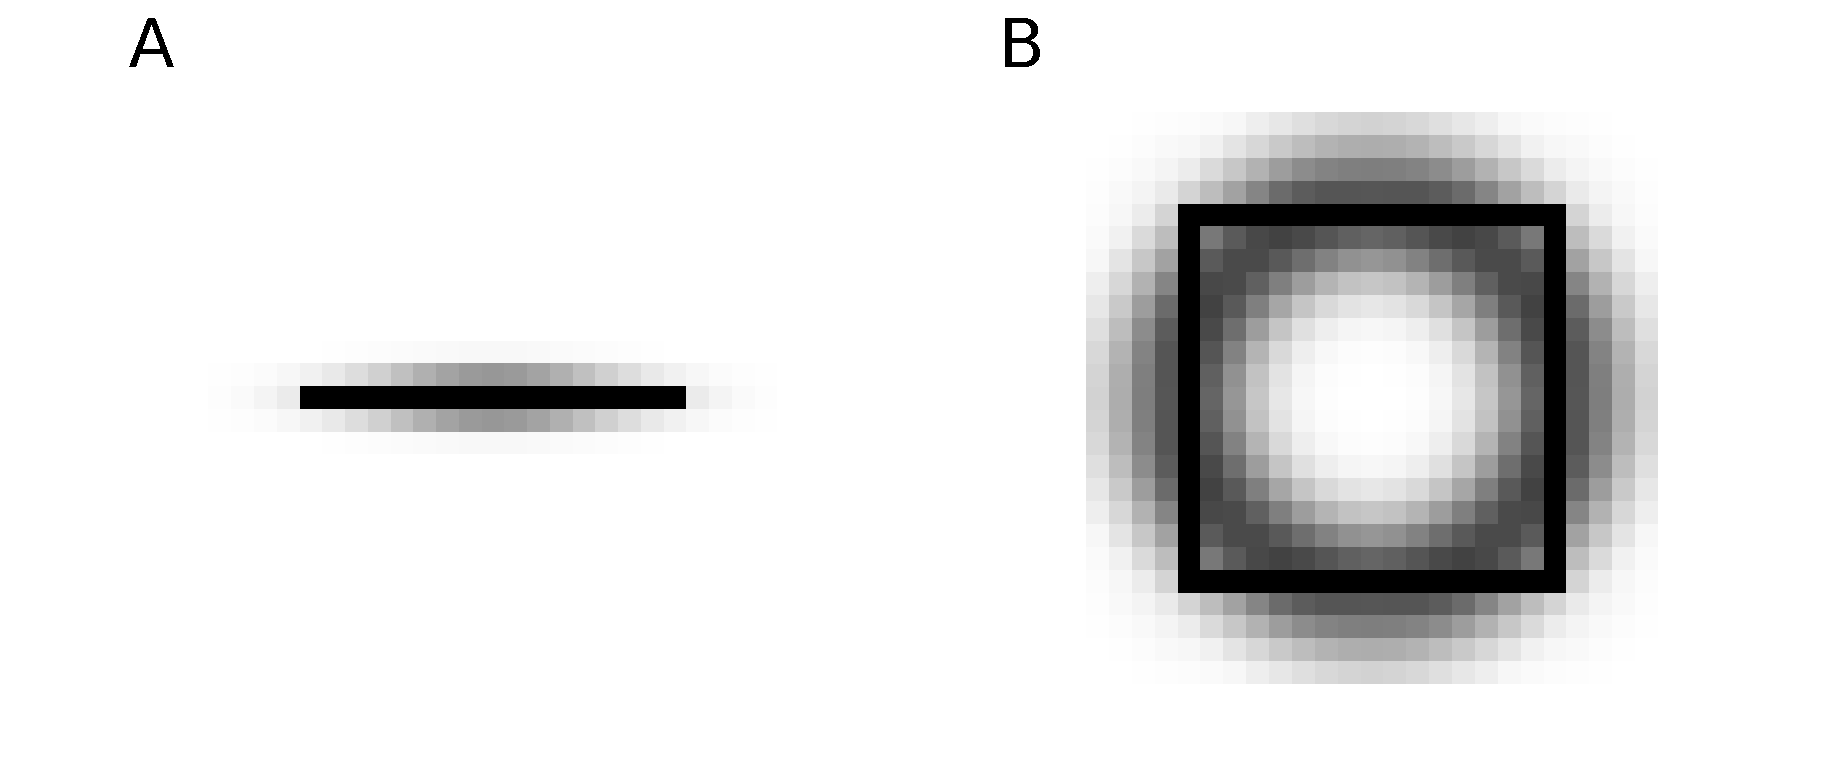
\includegraphics[width=0.75\textwidth]{Fig2.eps}
\end{center}
\caption{Spatial distribution of border ownership cell to grouping
  cell connectivity; darker pixels indicate stronger connection
  weights. A) Contour grouping neurons integrate features along
  oriented contours (horizontal line shown in black), emphasizing the
  Gestalt principle of good continuation. B) Object grouping neurons
  integrate features in a co-circular pattern (square figure shown in
  black), emphasizing the Gestalt principles of convexity and
  proximity.} 
\label{Fig:BG_projections}
\end{figure*}

%bh Describe key differences between our model and Stefan's model more explicitly here
Our approach is an extension of the 
%based on the 
%proto-
object-based model of perceptual organization proposed by
\cite{Mihalas_etal11b}. Different from their approach, we include a new population of contour grouping neurons to explain recent results on cortico-cortical interactions during contour integration~\citep{Chen_etal14}. As a result, top-down attention in our model can either be directed to grouping neurons representing contours or objects. Our model is also able to reproduce the time course of neural responses in different visual areas, while their model is based on mean neural activities. In order to create more complex input stimuli, we also increased the number of model orientations from two to four. As a simplification to their model, we only include one scale of grouping neurons since we focus on mechanisms that do not require multiple scales. 

%
%bh original Model Structure section
%Our approach is based on the 
%proto-object based model of perceptual organization proposed by
%\cite{Mihalas_etal11b} and extended to explain contour integration.
%We simplify their approach by only
%including one scale of grouping neurons rather than several, since we
%focus on mechanisms that do not require multiple scales. This
%simplification reduces the complexity of the model, including the
%number of neurons to be simulated. The model receives binary visual
%input, with the signal strength of the neuron whose preferred location
%and orientation coincides with the orientation of the stimulus bar at
%this location set to unity, and the activity of neurons
%coding for other orientations at this location set to zero.
%We use a total of four orientations,
%  $0, \pi/4, \pi/2,$ and  $3\pi/4$
% relative to the horizontal.
%
%Figure~\ref{Fig:anatomy} shows the overall structure of our model whose
%components are cortical areas V1, V2, and V4. 
%Each area is modeled as an $N_i\times N_i$ grid of neurons, where
%$N_i$ is the number of RFs in area $\rm V_i$. We
%choose $N_1=64$ for area V1, $ N_2=32$ for V2, and $N_4=8$ for V4, with
%neurons in higher areas having larger RFs~\citep{Poort_etal12}. At the level of V1, edge (E) cells receive direct input from the
%stimulus, see Figure~\ref{Fig:anatomy}. They activate other nearby
%E cells with the same orientation preference, and these lateral
%connections follow a one-dimensional Gaussian profile with a root-mean
%square (RMS) width eight times the receptive field size of an E cell
%(\ie, eight pixels
%in the input picture,
%where one pixel represents the typical size of the receptive field for E cells).
% E cells also activate local neighboring
%inhibitory (IE) cells,
%which are not orientation selective,
% and these connections are assumed to have a two-dimensional Gaussian
%weighting with a RMS width eight times the receptive field size of an
%E cell. IE cells then in turn inhibit all neighboring E cells with
%the same two dimensional Gaussian pattern. We do not model
%self-inhibition at any level of our model (\eg IE-IE connections)
%because we found that this was not needed to explain experimental
%results.
%
%At the level of V2, each E cell population activates two border
%ownership (B) cell populations with opposing border ownership
%preferences. 
%%en you haven't said what BOS is, except very briefly in the Intro
%%that is codes some relative position. So let's give an example:
%%bh ok
%For instance, E cells responding preferentially to a vertical line
%will project to two populations of B cells, one with a preferred border
%ownership selectivity for a foreground object located to the left of
%the vertical line, and the other preferring an object to its right.
%%
%B~cells of all orientations and border ownership selectivities
%project locally (with a 2D Gaussian spread of synaptic strength) to a
%population of inhibitory (IB) neurons. IB~cell 
%activity is therefore invariant with respect to border
%ownership as well as stimulus orientation. 
%These cells provide local inhibition of B cells.
%Connection patterns 
%within
%V2 mirror those in V1, 
%and the connections are assumed to follow a
%Gaussian distribution with a spread four times the receptive field
%size of a B cell.
%In addition, lateral connections exist between B
%cells with orthogonal orientation preferences, which help to transfer
%border ownership information along corners. 
%
%At the level of V4, B cells activate two different types of grouping
%cells. Contour grouping cells ($\rm G_c$) are
%orientation selective but not border ownership selective. They receive input from B cells with the
%corresponding preferred orientation and 
%both border ownership preferences.  
%These connections have an anisotropic two dimensional Gaussian
%distribution pattern, with an RMS width four times the receptive field size of
%a B cell parallel to the contour, and of 0.75 times the receptive
%field size of a B cell orthogonal to the contour, 
%see Figure~\ref{Fig:BG_projections}A.
%$\rm G_c$ cells are 
%most strongly activated by B cells 
%that share their orientation preference,
%and receive weaker inputs from B cells of other orientations.
% These connection strengths are tuned in order to explain the orientation
%dependence of contour grouping cells as observed experimentally
%\citep{Chen_etal14} and discussed in more detail below.
%Object grouping cells ($\rm G_o$) are sensitive to a co-circular
%arrangements of edges (with a radius eight times the receptive field
%size of a B cell) which  combines features of the Gestalt laws of good
%continuation, convexity of contour, and compact shape.  In other
%models
%\citep{Craft_etal07,Mihalas_etal11b,Ardila_etal12,Molin_etal13,Russell_etal14,Molin_etal15a,Hu_etal16a},
%the radii of the annuli spanned a range but as mentioned earlier, our
%interest was not on multi-scale processing but on the interaction of
%contours and objects.  Therefore we simplify our analysis by only
%considering one object size in this model.  $\rm G_o$ cells are
%maximally activated when an object of the chosen size is present at the location specific to each cell and activation decreases 
%gradually
%when object size or location deviates from the optimum.
%This is achieved by the pattern of the afferent input 
%(see Fig.~\ref{Fig:BG_projections}B)
%which, in contrast to $\rm G_c$ cells, only comes from B cells whose border
%ownership preference is consistent with such an object, see
%Figure~\ref{Fig:anatomy}.
%
%Each grouping cell projects back to exactly those border ownership
%cells from which it receives its input.  The grouping cells also
%project to edge (E) cells that co-activate with the border ownership
%cells that they receive input from with a similar pattern and
%strength.  Thus, the feedback from each grouping cell activates the
%same neurons that lead to its activation and also the neurons that are
%coactivated with the latter. 
%Object grouping neurons feed back to only those B neurons whose border ownership preference is consistent with the presence of
%an object at the location represented by the object grouping
%neuron. It is this difference in feedback that generates
%border ownership selectivity in B neurons (\ie the difference in responses
%between $B_L$ and $B_R$ neurons in Figure~\ref{Fig:anatomy}).  In
%contrast, responses of E cells are not border ownership selective since
%their bottom up input depends only on the local orientation, and 
%feedback to them
%is from object grouping cells on {\em both}
%sides of the local contour.
%%en slightly simplified:
%%(feedback from only one side is shown in Figure~\ref{Fig:anatomy}).  
%%(Figure~\ref{Fig:anatomy} only shows feedback from one side). 
% 
%%en I know you want to get this out (me too!) but I wonder if it would
%%be better to add another G_o cell in Fig 1. To the right of the
%%existing figure. It would have only connections to the IG_r, B_R and
%%E cells. I think the current figure is confusing, even though we have
%%the parenthesis in the previous sentence, since it implies that
%%the pattern shown is be repeated (tiled) which is not the case. 
%%
%%bh edited figure for this new version that shows G_o cells on both sides
%
%As mentioned previously, the feedback
%from grouping cells to border ownership cells is modulatory, rather
%than driving. 
%This is implemented in the framework of the neuron model given by
%Eq.~\ref{eq:1} 
%with feedback from grouping cells acting as additive input to edge and
%border ownership cells, and  the local circuitry within each area
%transforming this input into a quasi-multiplicative
%effect.
%The underlying mechanism is explained by \cite{Mihalas_etal11b}. Briefly, 
%in the absence of sensory input, the
%direct excitatory input from grouping cells to E and B cells is
%compensated by the sum of all local inhibitory input from IE and IB
%cells; feedback therefore does not modify the activities of cells that
%do not receive sensory input.
%On the other hand, 
%when sensory input is present, E and B
%cells receive bottom-up excitation that is no longer balanced by the
%inhibition, thus allowing for further modulation of activity via
%feedback or attention. 
%Another
%model of modulatory feedback from grouping
%cells to border ownership cells which is based on NMDA-type 
%feedback connections was recently developed \citep{Wagatsuma_etal16a}.
%
%All G cells also activate inhibitory grouping (IG) cells, which have
%both an orientation and side-of-object preference (akin to that of B
%cells). IG cells implement competition between the different possible
%interpretations of a visual scene in terms of proto-objects. 
%The input from G cells
%to IG cells has a connection pattern and strength similar to the
%feedback
%from (both types of) G cells 
% to excitatory border ownership neurons.  IG cells inhibit all
%${\rm G_c}$ cells nonspecifically, as well as  ${\rm G_o}$ cells that do not
%match their side of figure preference. The pattern of inhibition is
%assumed to follow a two-dimensional Gaussian distribution, with RMS
%equal to the receptive field size of a G cell along the preferred
%orientation of the IG cell, and half this 
%RMS orthogonal to the preferred orientation.
%
%Attention is often considered as a ``spotlight'' that selects a
%certain region of the visual input 
%%en added:
%%bh ok
%\citep{Eriksen_StJames86}.
%In its simplest form, this could
%be implemented by boosting the activity of feature-coding neurons
%within the attended region (the E cells in our model). This purely
%spatial allocation of attention can not explain 
%that observers can selectively attend
%to objects \citep{Duncan84,Egly_etal94,Scholl01}. Following \cite{Craft_etal07}
%and \cite{Mihalas_etal11b}, attention in our model is therefore
%implemented in the form of additional input to grouping cells, whose
%activity represents the presence of proto-objects or contours,
% as shown in Figure~\ref{Fig:anatomy}. This attentional input is
% relatively weak; 
%we selected its strength as 7\% of that of the driving input from the
%sensory (E) cells.  

\subsection{Model Implementation}
\label{sec:implementation}
Model neuronal populations (usually referred to as ``neurons'' in the
following) are represented  by their mean  activity (rate coding). 
The activity is determined by a set of
coupled, first-order nonlinear ordinary differential equations which
was solved in MATLAB (MathWorks, Natick MA) using standard numerical
integration methods. 
The mean firing rate is necessarily positive, therefore units
are simple zero-threshold, linear
neurons which receive excitatory and inhibitory current inputs with
their dynamics described by,
\begin{equation}
\label{eq:1}
\tau f'(t) = -f + \left[ \sum W \right]_{+}
\end{equation}
where $f$ represents the neuron's activity level and $\tau$ its time
constant, chosen as $\tau$ = $10^{-2}$ s for all neurons,
 the sum is over all $W$ which are the neuron's inputs, 
%
$f'$ is the first derivative of $f$ with respect to
time, and $[\,]_{+}$ means half-wave rectification.

All simulations were performed on a 
300-core CPU cluster running Rocks 6.2 (Sidewinder), a Linux
distribution intended for high-performance computing.  A total of 100
simulations were performed for each experimental condition, and our
results are based on the mean neural activities averaged over these
simulations with different randomly selected stimulus noise patterns, see
sections~\ref{sec:contour_exp} and~\ref{sec:FGO}.

To constrain our model parameters, we used two sets of
neurophysiological data. The first comes from recent contour grouping
results~\citep{Chen_etal14}, and our model was able to largely
reproduce the magnitude and time course of contour integration at both
the V1 and V4 levels. The second set of results comes from studies on
border ownership~\citep{Qiu_etal07}, specifically the 
vector
modulation index at the V2 level
(see section~\ref{sec:vmi})
 in the presence and absence of
attention. In order to fit the model parameters, we started from the
parameters given by \cite{Mihalas_etal11b}, and modified them to fit
the larger body of experimental results to include contour
integration, border ownership selectivity, and attentional selection. 
We note that the original parameters already fit the
model quite well.

\subsection{Contour integration experiments} 
\label{sec:contour_exp}
For the contour integration experiments reported by
\cite{Chen_etal14}, awake behaving
 monkeys were trained to perform a two-alternative
forced-choice task using two simultaneously presented patterns, one
containing a contour embedded in noise and one that was noise only
(see Figure~\ref{Fig:Contour_Results} for examples). 
The patterns
were composed of 
$0.25^{\circ}$ by $0.05^{\circ}$
bars distributed in $0.5^{\circ}$ by $0.5^{\circ}$ grids. 
The diameter
of the patterns was $4.5^{\circ}$, and the number of bars in the
embedded contour was randomly set to 1, 3, 5, or 7 bars within a block
of trials in order to control the saliency of the contour.
To obtain a reward, the
monkey had to saccade to the pattern containing the contour, 
with the location of the stimulus containing the contour as well as the number
of collinear bars making up the contour  changing between trials. 
 When the number of bars was set to 1, both presented stimuli were noise patterns, and the monkey had to guess at a chance level of 50\%. 
 While the animals were performing the task, simultaneous
single- or multi-unit recordings were made in area V1 and V4 neurons with
overlapping receptive fields. 

We modeled these experiments by creating visual stimuli
contained in a $4.5^{\circ}$ by $4.5^{\circ}$ area
as in the~\cite{Chen_etal14}  study. This area was projected onto
a V1 layer of $64 \times 64$ neurons, each with a receptive field
size of $\sim0.7^{\circ}$  
so the receptive fields overlapped ten-fold at each location in the visual
field. 
We divided the input field into a $9 \times 9$ grid (each grid point
at the center of a $0.5^{\circ}$ by $0.5^{\circ}$ area)
and we placed at each grid location a
stimulus bar of size $\sim0.21^{\circ}$ by $\sim0.07^{\circ}$ 
(so the bar consisted of three adjacent pixels).
Each stimulus bar had one of four orientations, 
$0, \pi/4, \pi/2,$ or $3\pi/4$. 
We always positioned the
contour at the center of the  
visual field,
and we changed the length of the
contour by adding bars to either end 
 of the contour. We
``recorded'' from the V1 receptive field that was at the center of the
stimulus (marked by the yellow circles in Figure~\ref{Fig:Contour_Results}),
as well as from the corresponding V4 neuron.
Due to their size, V4 receptive fields
basically enclosed the entire
contour.

\begin{figure*}
\begin{center}
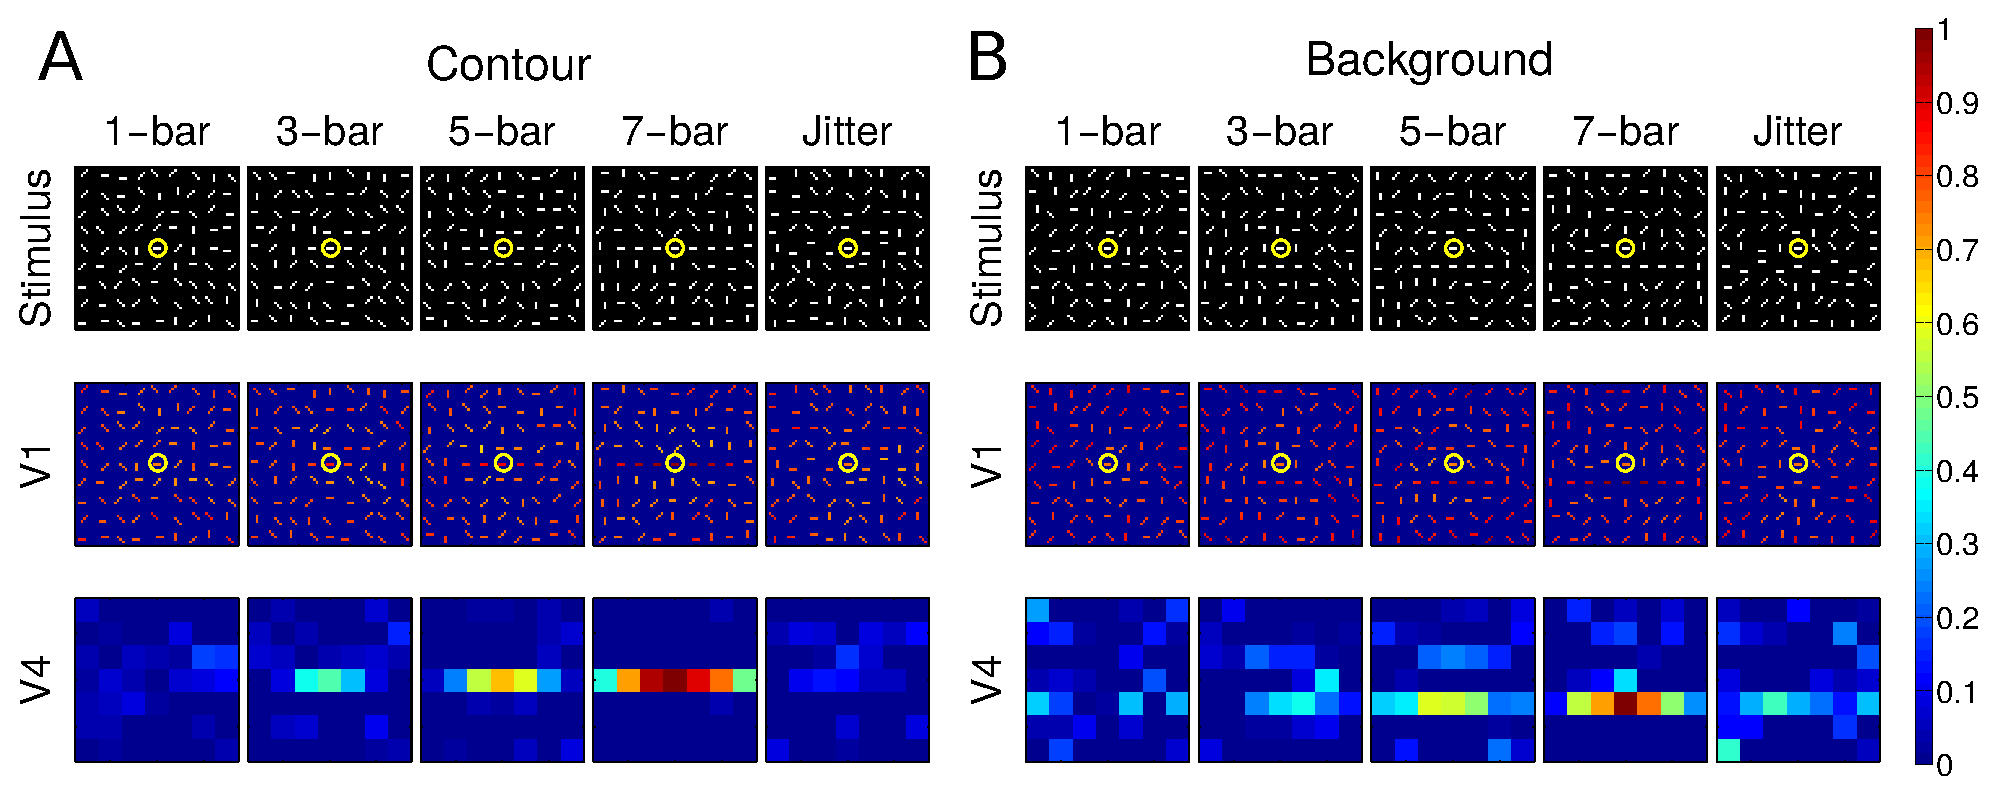
\includegraphics[width=0.75\textwidth]{Fig3.eps}
\end{center}
\caption{Normalized V1 $E$ cell and V4 $G_c$ cell population responses
 to contours of
varying lengths in either the contour (A) or the background (B)
condition. In (A), the ``recorded'' neuron is on the contour; in
(B), it is offset from the contour. The top row shows stimuli, the
second and third rows show activity in model areas 
V1 and V4, respectively. Yellow circles mark the RFs of the V1 neurons whose activity is shown in Figure~\ref{Fig:Neural_responses}.
Activity from model area V2 is not shown because a single contour does not produce clear border ownership selectivity, and the activity in V2 is essentially the same as that in V1, but with reduced spatial resolution due to the lower number of neurons. 
Columns in each condition show, from left to right, increasing
contour length, with the right-most column showing a jittered stimulus configuration (see text). Neural
activity is color coded
and normalized to the 7-bar stimulus in both contour and background conditions,
 with warmer colors representing higher
activity (see color bar at right). 
%Both V1 and V4 responses increased with contour length, with the
%increase being much smaller in V1 (not easily visible in the color coding)
%than in V4.
}
\label{Fig:Contour_Results}
\end{figure*}

\subsection{Figure-ground segregation experiments} 
\label{sec:FGO}
For the figure-ground segregation experiments~\citep{Zhou_etal00,
  Qiu_etal07, Zhang_vonderHeydt10},
 awake, behaving monkeys were trained on a fixation task. 
Receptive fields of each recorded 
neuron in areas V1 and
V2 were first mapped to determine the optimal stimulus properties for
that neuron. Afterwards, 
in some experiments, 
a square shape was presented on a uniform
gray background with one edge of the square centered on the receptive
field of the neuron at the neuron's preferred orientation.  
In other
experiments (results shown in
Figures~\ref{Fig:Overlap_Square_exp_model} and~\ref{Fig:Overlap_Square})
the stimulus consisted of two 
partially overlapping squares, and again the receptive field of the
recorded neuron was centered at its preferred orientation on one edge
of one of the squares.  
The size of the square varied between experiments but it was always chosen such
that the closest corner was far away from the classical receptive
field of the recorded neuron. The square was presented in two
positions between which it was ``flipped'' along the long axis of the
neuron's receptive field. For instance, if the preferred orientation
was vertical, the square was presented either to the left or the right
of the cell's receptive field (we used this example in the choice of
the indices in Figure~\ref{Fig:anatomy}).  The difference in the
firing rate of the neuron for when the square appears on one side
versus the other side is known as border ownership
selectivity. Importantly, in all stimulus conditions, local contrast
within the receptive field of the neuron remained the same between
these two conditions; only global context information about the side
of the square changed, so the neuron had to integrate information from
outside its classical receptive field.

We modeled these experiments by creating visual stimuli that were
projected onto the V1 layer. The input to the simulation was 
either a single square of a size that maximally activated $\rm G_o$ grouping cells of
the size chosen in our model,
or two partially overlapping squares, as shown in
Figure~\ref{Fig:Overlap_Square}, 
with each of these squares having the same
optimal size. 
In more general models, as in those
cited in section~\ref{sec:implementation}, grouping cells of many
scales are present, covering the range of possible objects in the
input. We calculated border ownership selectivity at the V2 level
using the vector modulation index defined in section~\ref{sec:vmi}.
In order to create noisy versions of the
single
square image
(Figure~\ref{Fig:Square}, bottom row),
 we followed a
similar approach as in the contour integration experiments.  We again
divided the visual field into a $9 \times 9$ grid and we positioned
horizontal and vertical bars at specific grid points to generate a
square. We then placed a stimulus bar at all other grid points, with
their orientations randomly chosen from four possibilities,
$0, \pi/4, \pi/2,$ and $3\pi/4$.

\subsection{Quantitative assessment of border ownership selectivity:\\
  Vector modulation index}
\label{sec:vmi}
The strength of border ownership selectivity was quantified using the
vector modulation index, introduced by \cite{Craft_etal07} and defined
by the expression 
\begin{equation}
\label{eq:2}
\vec{v}(x,y) = m_{\hat{\imath}}(x,y)\hat{\imath} + m_{\hat{\jmath}}(x,y)\hat{\jmath}
\end{equation}
where $\hat{\imath}$ and $\hat{\jmath}$ are unit vectors along the horizontal and vertical image
axis, respectively, and the components $m_{\hat{\imath}}(x,y)$ and $m_{\hat{\jmath}}(x,y)$ are the usual modulation indices along their respective axes, defined as
\begin{equation}
\label{eq:3}
\begin{split}
	m_{\hat{\imath}}(x,y) = \frac{\sum_{\theta}
        B_{\theta}(x,y)\cos\theta}{\sum_{\theta}
                \left|B_{\theta}(x,y)\cos\theta\right|} \\
	m_{\hat{\jmath}}(x,y) = \frac{\sum_{\theta}
        B_{\theta}(x,y)\sin\theta}{\sum_{\theta}
                \left|B_{\theta}(x,y)\sin\theta\right|}
\end{split}
\end{equation}
where $B_{\theta}(x,y)$ is the border ownership signal (difference between
the activities of the two opposing B neurons) at the preferred
orientation $\theta$ at position $(x,y)$, and $\theta$ runs over all
angles taken into account in the model 
(four directed orientations in our case, namely $0, \pi/4, \pi/2,$
and $3\pi/4$, each with both side-of-figure preferences). The sums in the denominators are over absolute values.

Both components in Eq.~\ref{eq:3} are limited to values between +1 and
-1. For the x-component, for instance, a positive value of
$m_{\hat{\imath}}(x,y)$ signifies that the figure is to the right of
position (x,y) and a negative value signifies that the figure is to
the left. Its absolute value indicates the ``strength'' of the
border-ownership signal, with zero being equivalent to ambivalence
between left and right. The corresponding comments also apply to the
y-component, $m_{\hat{\jmath}}(x,y)$, regarding the figure's position
upward or downward of (x,y). The direction of the vectorial modulation
index $\vec{v}(x,y)$ defined in Eq.~\ref{eq:2} indicates the position
of the foreground figure in the two-dimensional image plane relative to
the point (x,y). For instance, positive values in both components
[$m_{\hat{\imath}}(x,y) > 0$, $m_{\hat{\jmath}}(x,y) > 0$] indicate
that the figure is located upwards and to the right of (x,y).  

\begin{figure*}
\begin{center}
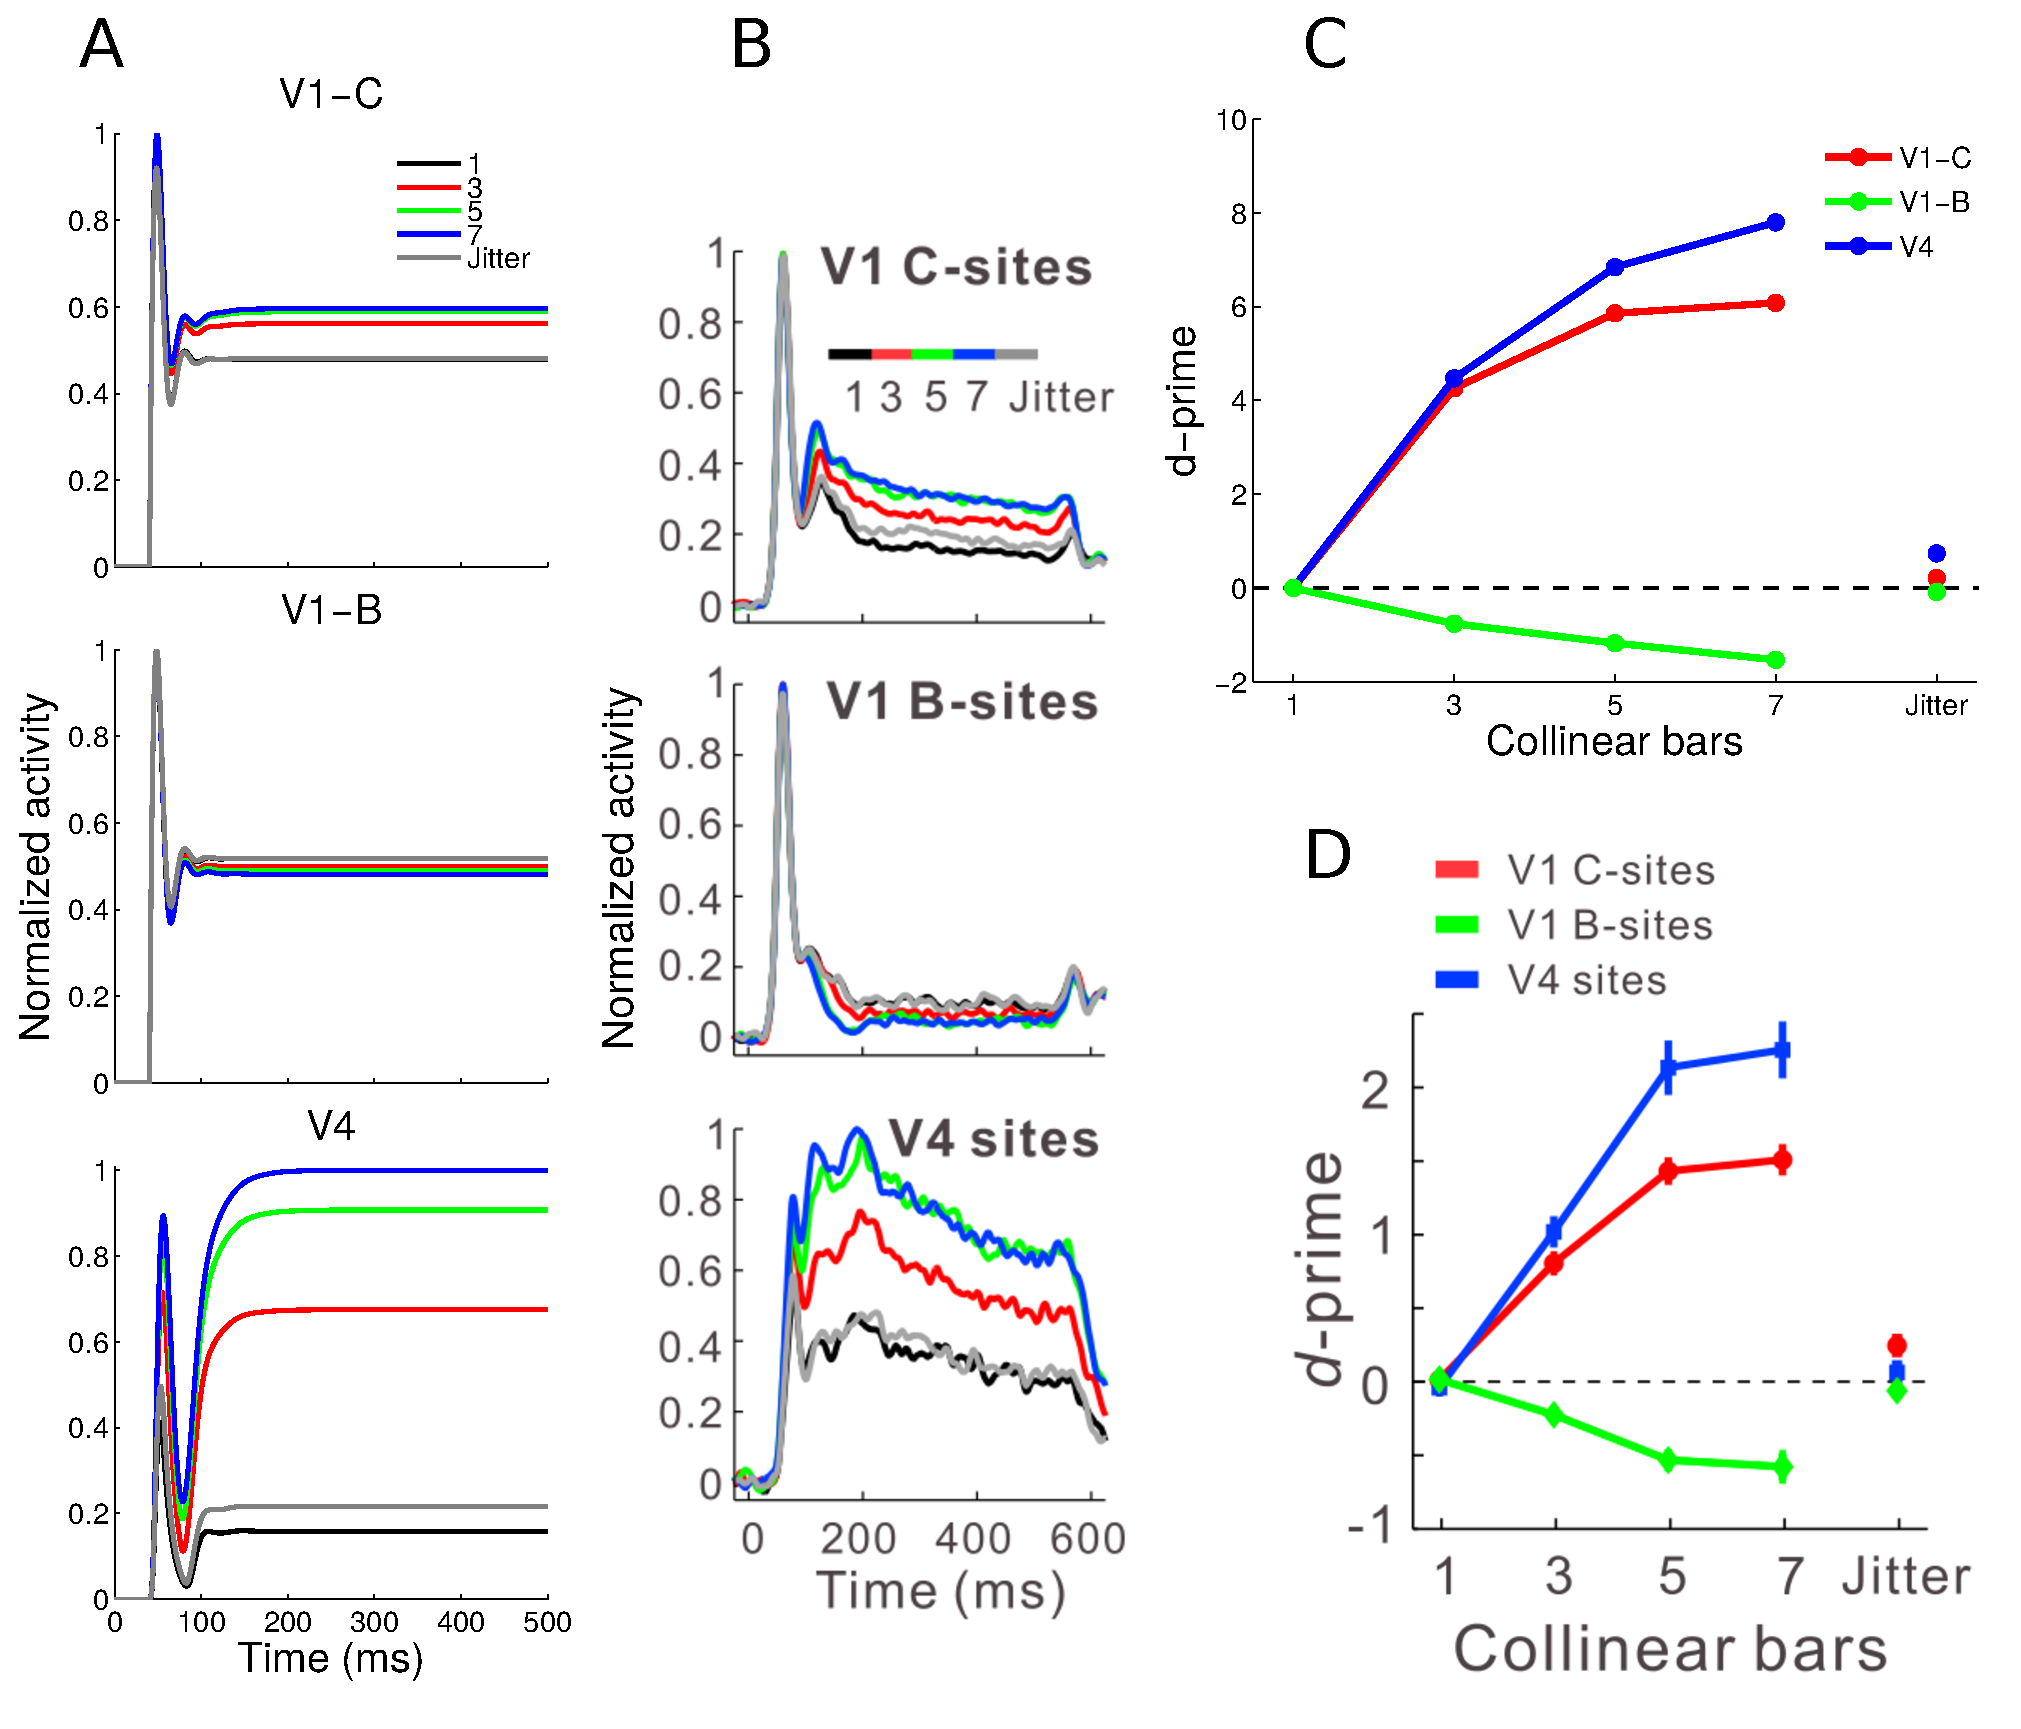
\includegraphics[width=0.75\textwidth]{Fig4.eps}
\end{center}
\caption{Normalized V1 $E$ cell (contour and background sites) and V4
  $G_c$ cell neuronal activity and contour-response $d'$ to contours of
  varying lengths. (A) V1 contour (top) and background (middle) sites
  and V4 sites (bottom) showed facilitation followed by saturation
  with increasing contour length (see legend). V1 background sites
  showed greater suppression with longer contours. The jitter
  condition involved a 7-bar pattern where each bar was laterally
  offset to disrupt collinearity. (B) Corresponding experimental
  observations showing normalized and averaged PSTHs from
  the~\cite{Chen_etal14} study. 
%  This panel was adapted from Figure~2A
%  of their paper. 
  (C) Contour-response $d'$ was higher for the V4
  sites compared to the V1 contour sites, and was facilitated by
  increasing contour length. V1 background sites had increasingly
  negative $d'$ with longer contours, indicating background
  suppression. The jitter condition reduced the absolute value of the
  $d'$ values to close to zero, making it similar to the baseline
  noise condition. (D) Corresponding experimental observations,
  showing the mean contour-response $d'$ from the~\cite{Chen_etal14}
  study. 
%  This panel was adapted from Figure~2F of their paper.
  Panels B and D are modified from Figure~2 of~\cite{Chen_etal14}.
  All model results (neural responses and contour-response $d'$) are
  averages for a single neuron over 100 simulations.
}
\label{Fig:Neural_responses}
\end{figure*}

\section{Results}
\label{sec:results}
\subsection{Contour enhancement in V1 and V4}
We examined contour-related responses in our model using visual
stimuli composed of collinear bars among randomly oriented bars
(Figure~\ref{Fig:Contour_Results}), closely matching the stimuli used
in the physiological experiments by \cite{Chen_etal14}. The number of
collinear bars constituting an embedded contour
was set to either 1, 3, 5, or 7 bars, 
determining the length
of the embedded contour, 
which also controlled its saliency.
When the number of collinear bars was one, the stimulus was identical to a
noise pattern. We compared the activity of model neurons
whose RFs are centered on the contours 
or in the noise background (but close to contours)
with that obtained in the analogous positions during
neurophysiological recordings.

V1 responses were split into those of neurons on contour sites
(C-sites) and background sites (B-sites). For contour sites
(Figure~\ref{Fig:Contour_Results}A), the embedded
contour was centered on the RF of a neuron with a preferred
orientation matching that of the contour. For background sites, the
contour was laterally placed 0.5$^{\circ}$ away from the RF center of the recorded neuron, and a background bar was placed in the RF
(Figure~\ref{Fig:Contour_Results}B), with the contour orientation
again matching the preferred orientation of the recorded neuron.
%bh Additional note on Figure 3, as one reviewer did not think we mentioned it enough in terms of the results. Maybe we can add more here?
Both V1 and V4 neurons along the contour showed increased activity with contour length. Neurons on the background showed increased suppression with contour length.
%
Correspondingly, we 
%also
 show in Figure~\ref{Fig:Neural_responses} the
responses of neurons whose preferred orientations align with the
contours
%bh added
 (yellow circles in Figure~\ref{Fig:Contour_Results}).
%

Except for an input delay of 40ms corresponding to the duration of
visual processing from the retina to V1, we did not explicitly model
any time delays in the feedforward or feedback connections of
our model, as we were not attempting to reproduce 
any specific latency effects.
Nevertheless, our model generally reproduced the dynamics of neural
responses to contours in both V1 and V4 observed in the
\cite{Chen_etal14} experiment (Figure~\ref{Fig:Neural_responses}A).
The most salient feature of the neuronal responses is that the levels
of sustained activity differ based on the number of bars in the
embedded contour. This is observed both for contour sites and for
background sites but, importantly, this effect went in opposite
directions for these two cases.  As the number of collinear bars
increased from one to seven, V1 contour sites centered on the contour
showed increased activity, with response saturation after five
bars. In contrast, V1 background sites that were offset from the
embedded contour showed a decrease in activity with increasing number
of bars in the background (response suppression). Similar to V1
contour sites, V4 sites showed saturating responses with increasing
contour lengths (Figure~\ref{Fig:Neural_responses}A, bottom).  These
results were qualitatively similar to those obtained in
the~\cite{Chen_etal14} experiments which are reproduced in
Figure~\ref{Fig:Neural_responses}B (their Figure~2A).
%
\begin{figure*}
\begin{center}
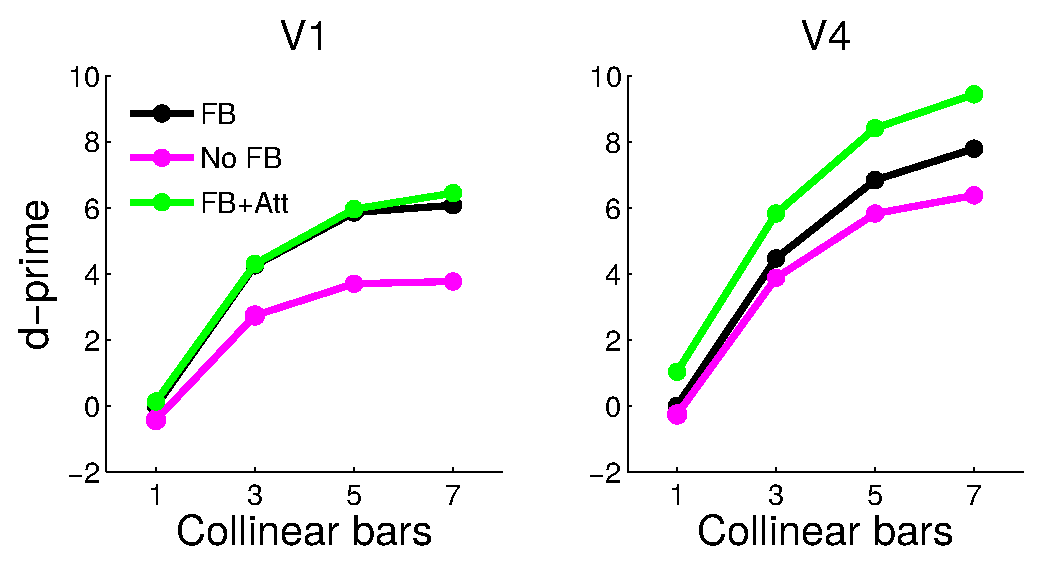
\includegraphics[width=0.75\textwidth]{Fig5.eps}
\end{center}
\caption{Contour-response $d'$ in V1 $E$ cells (A) and V4 $G_c$ cells (B) for the model with (green) and without attention (black), and for the model with feedback removed 
%bh changed to magenta for JNeuro color considerations
%(red).
(magenta). Attention strongly increased
  contour-response $d'$ in V4 (B), while the lack of feedback strongly
  decreased contour-response $d'$ in V1 (A).}
\label{Fig:FB_att}
\end{figure*}
%

The model data also showed strong onset transients in both (contour
and background) V1 populations (Figure~\ref{Fig:Neural_responses}A,
top and center), again in good agreement with experimental results
(Figure~\ref{Fig:Neural_responses}B, top and center). Transients in V4
neurons were weaker, in both model and experimental data, and nearly
absent in the experimental data (though not the model) for longer
contours (Figure~\ref{Fig:Neural_responses}B, bottom).
%
%bh commented out, there is overshoot in V4 for contours of shorter length (e.g. 1-bar, 3-bar) and does not seem to be a necessary detail
%
%To understand the origin of the  difference between
%model results and experimental data in V4, we observe that in V4 (but
%not in V1), the transient does not consist of an overshoot. Instead, 
%the peak of the initial activity spike is at a similar level
%as the later sustained activity (which, after a few hundred
%milliseconds, decays further but our model does not address dynamics
%at such long time scales). 
%
The transient peak observed in the model results
is due to a sharp suppression of the activity level for a short
($<50$ms) period which is not observed in the empirical data. We
believe that this suppression is due to the  strong inhibition at the
V4 level between G and IG cells, without equivalent
excitation between different G cells.
%bh commented out, one reviewer did not like our speculation about the underlying circuitry
% Such mutual excitation may exist
%in biological cortex and help to counteract the
%observed suppression after the initial transient.
%en I would think the reviewers will ask why we don't add such
%excitation in the model if we think it can explain the data
%better. What is your response?
%
%bh I think your description above is very good. I also thought about
%this some more, and I think there are a couple of other possible
%explanations: 
%
%1) essentially each level of the model (V1, V2, and V4) produces a
%low-passed version of the previous level's output. If a strong
%transient occurs in V1/V2 (which the data seems to show), then it
%should also be passed onto V4 by virtue of the dynamics of the
%system. 
%2) there is no self-inhibition in the model, which may work to reduce
%the suppressive effect of the inhibitory cell population at each
%level 
%
%V4 may counteract this strong initial transient by some mechanism
%that we currently have not modeled- e.g. self-inhibition, longer time
%constants, saturation, lateral excitation, etc. In terms of
%responding to this potential critique of just adding the lateral
%excitation, it could be done but may require additional parameter
%tuning (I haven't really tested it). Arguments against it would be
%that not having it makes the model more simple, and also, in Stefan's
%original model there was no excitation between grouping cells. Also,
%I'm not sure we can rule out other ways the system may eliminate this
%initial transient (i.e. using lateral excitation may only be one
%possiblity). 
%en OK, let's leave these comments in here, in case we need them to
%address reviewers' concerns.

%%bh One reviewer did not see the value in referencing this work, so I commented it out for now. Anyways, the reader has to take our word for it, since we don't show these results from Chen et al which we are referencing. I think our statement above is concise and to-the-point about why we observe strong initial transients in V4
%
%It is also interesting to note that in a separate set of
% experiments, which were used to test contextual
%influences outside the classical RF in  V4, \cite{Chen_etal14} found
%that neurons showed much stronger initial transients (their Figure~4, not shown here).
%In these experiments, much larger
%stimuli were used (50$^{\circ}$ in diameter rather than
%4.5$^{\circ}$).
%One explanation for the initial transient in V4
%responses in these experiments is that the larger stimuli 
%caused general surround suppression of V4 responses.
% Contour facilitation at the V4 level then
%acted on top of this general suppression, which gave rise to the
%initial transient and later different levels of sustained responses
%depending on the length of the contour.

Following \cite{Chen_etal14}, 
we quantitatively analyzed the contour responses using the d-prime
$(d')$ metric from signal detection theory~\citep{Green_Swets66}, which
is based on the difference in distributions of mean neuronal firing
rates between a contour pattern and the noise pattern integrated over
the whole interval shown in Figure~\ref{Fig:Neural_responses}A,B, \ie
0-500 ms.  Neuronal responses to the 1-bar pattern (the noise pattern)
were the baseline for examining contour-related responses in V1 and
V4, this pattern therefore had a contour-response $d'$ of zero. The
contour-response $d'$ increased with contour length for both the V1
contour and V4 sites, and $d'$ decreased with contour length for the V1
background sites, Figure~\ref{Fig:Neural_responses}C.

The agreement between model (Figure~\ref{Fig:Neural_responses}C) and
experimental results (Figure~\ref{Fig:Neural_responses}D) is striking.
One difference we note is that the absolute values of all model $d'$
substantially 
exceeded the corresponding experimental values. 
This is to be expected since
no noise was included in the model (other than the random orientation of input
stimulus bars which is also present in the experimental approach)
while there were surely multiple sources of noise in the biological
system. While we have not thoroughly investigated this question, it is
likely that addition of noise to the model will decrease the $d'$
values.

\begin{figure*}
\begin{center}
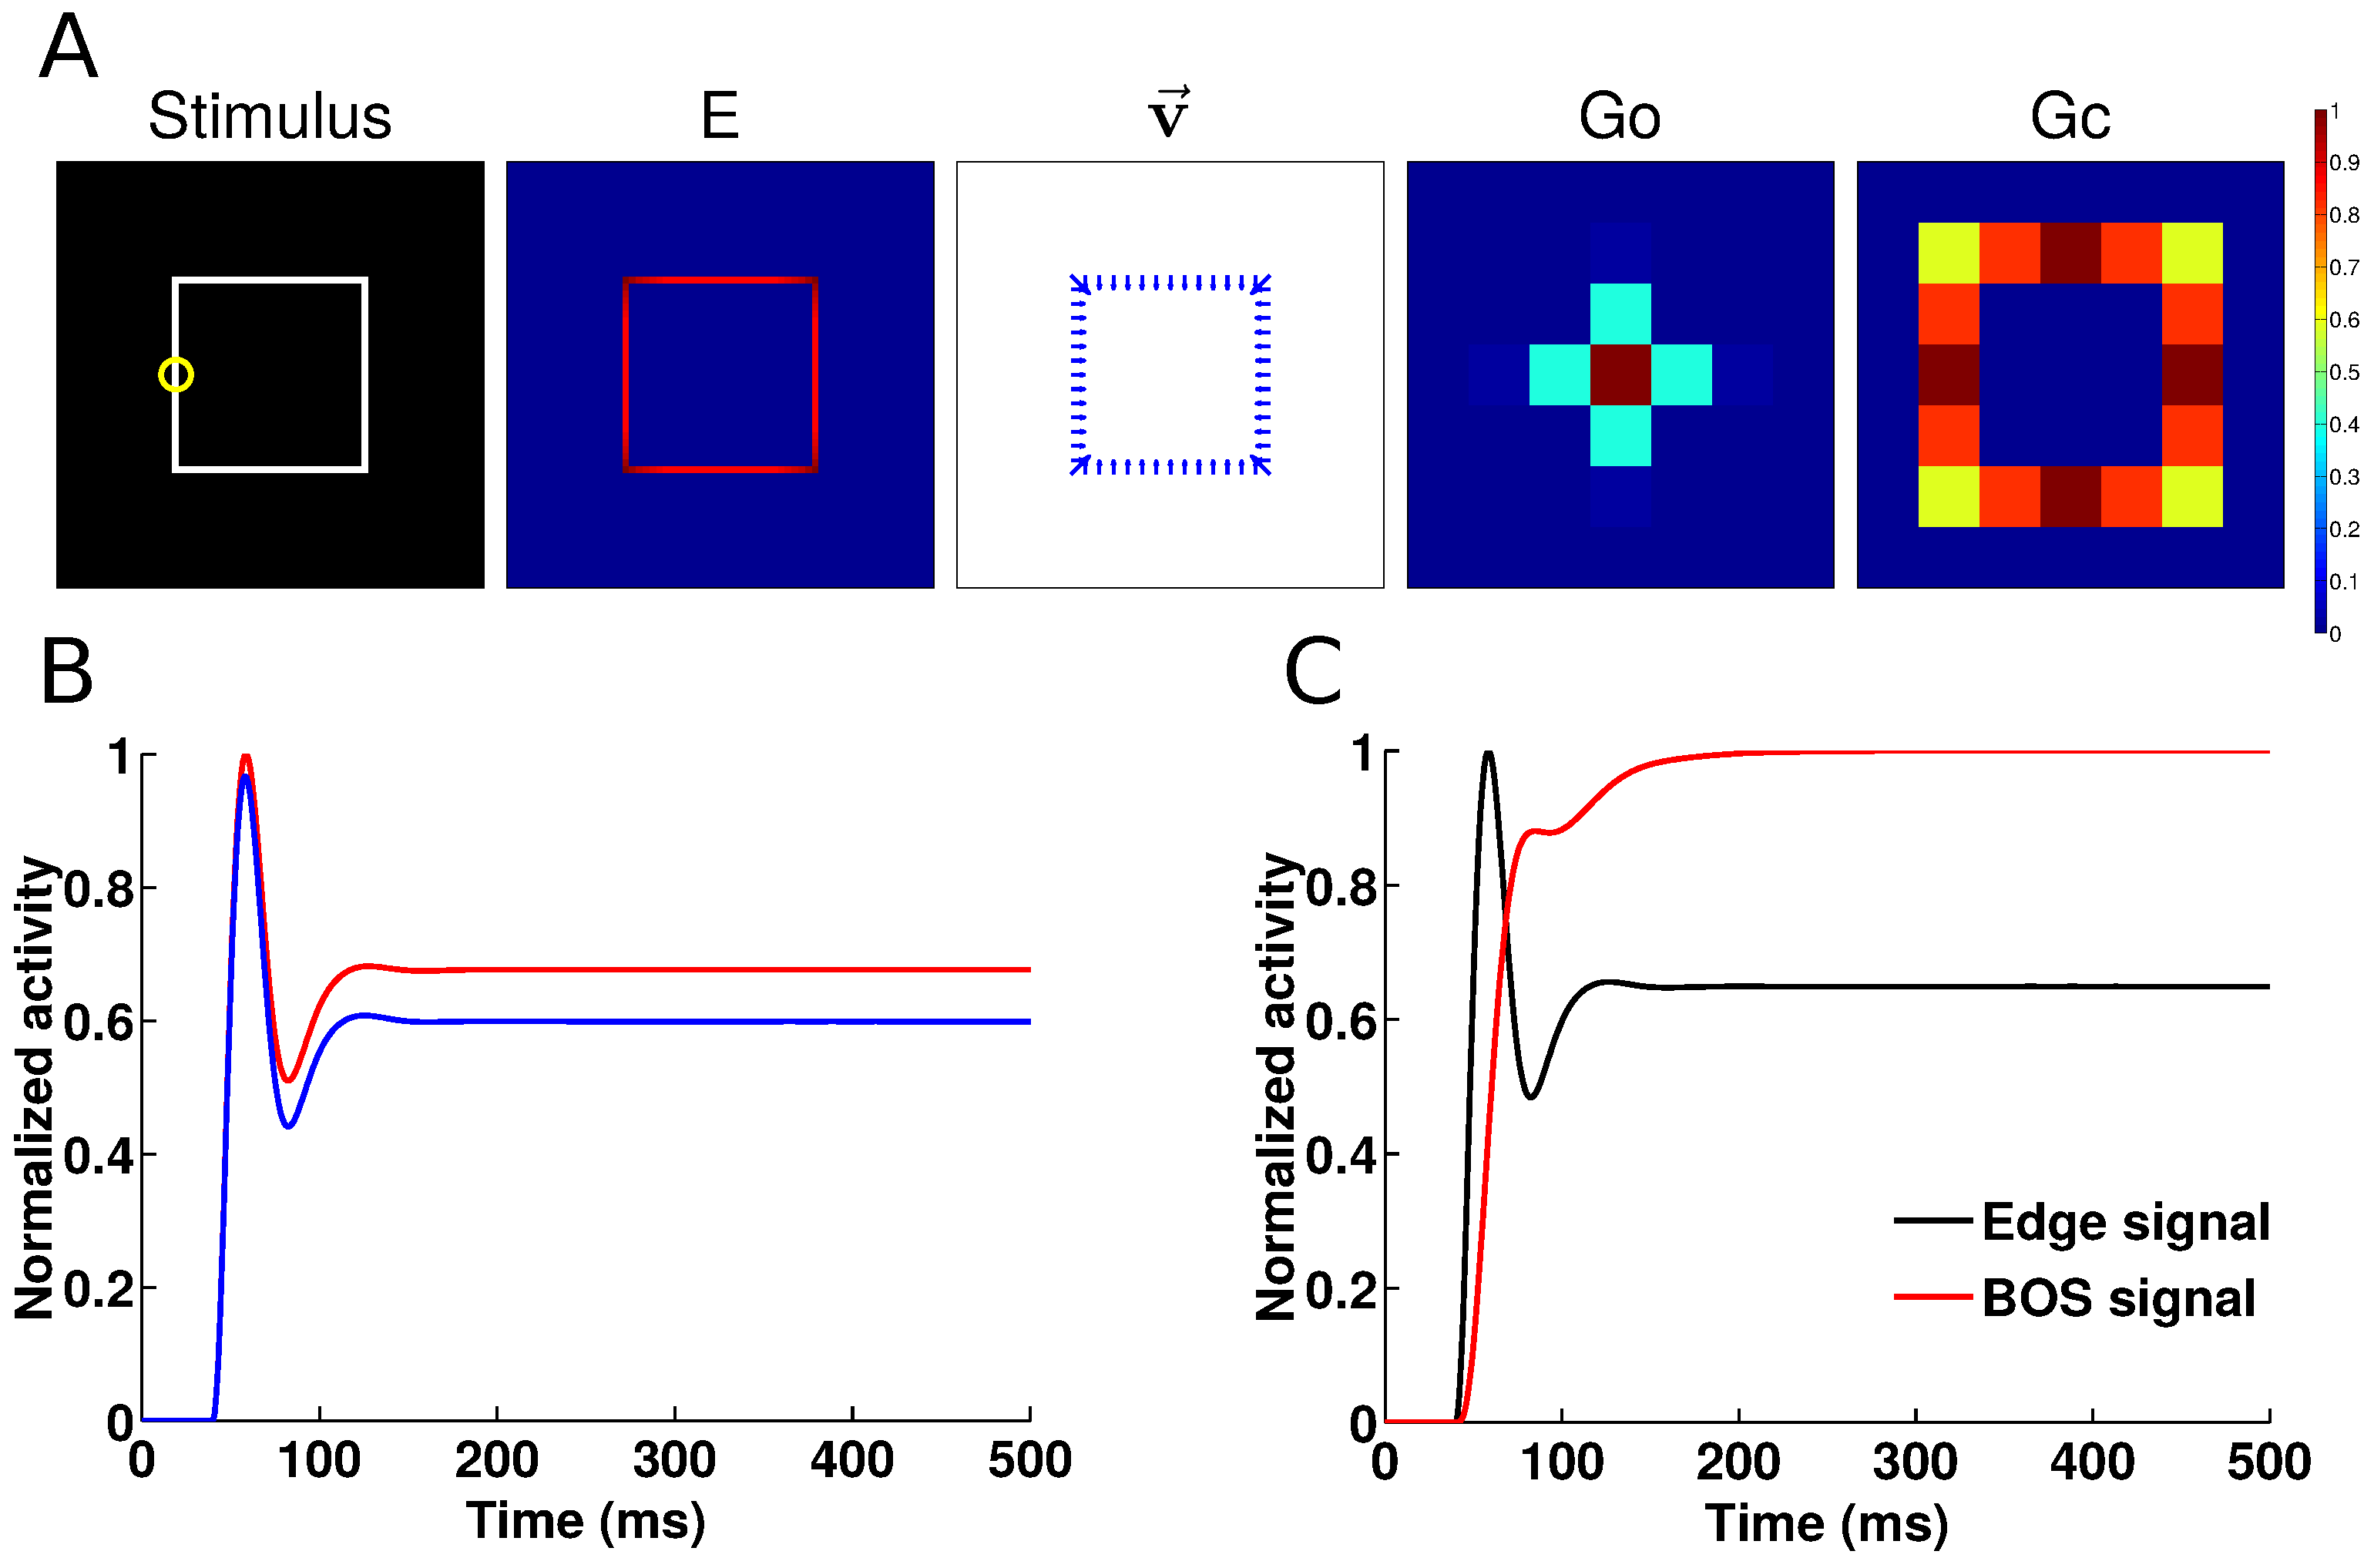
\includegraphics[width=0.75\textwidth]{Fig6.eps}
\end{center}
\caption{Figure-ground segregation of a square object with (bottom
  row) and without (top row) noise. Shown are (left to right) the input
  stimulus, the edge cell activity (E), the border ownership
  assignment along edges (shown as the vector modulation index $\vec{v}$,
  section~\ref{sec:vmi}), the object grouping 
  neuron activity 
$(G_o)$
 and the contour grouping activity
$(G_c)$.
 Activities are normalized within each map, and warmer colors
  indicate higher activity (see color bar at right).}
\label{Fig:Square}
\end{figure*}

At first sight, it seems possible that 
V4 neurons respond with a higher firing rate to longer contours than
to shorter ones simply as a consequence of 
the large size of RFs in V4. 
In this view, the enhanced responses in V4 with increasing contour
length is due to the spatial summation of many bars
within the RF at the optimal orientation,
independent of their precise location in the RF. 
To  investigate this possiblity,
~\cite{Chen_etal14} introduced a ``jitter'' condition to the 7-bar
contour, where the collinear bars were laterally offset 
by a small amount (much less than the receptive field size)
in an alternating pattern, in order to disrupt the collinearity of the original contour. They showed that jittering disrupted the
contour integration process and reduced the neural responses in V1
and V4 close to baseline levels (Figure~\ref{Fig:Neural_responses}B,
gray lines). We found the same result in our model,
Figure~\ref{Fig:Neural_responses}A, gray lines.  Furthermore, in the
jitter condition, contour-response $d'$ approached baseline for the
V1 and V4 sites, as shown in the rightmost points for
Figure~\ref{Fig:Neural_responses}D for experimental data and
Figure~\ref{Fig:Neural_responses}C for model results. In both cases,
no substantial difference between the jitter condition and the
baseline noise condition was observed.

We also investigated the orientation and position dependence of contour-related responses in V1 and V4, and found close agreement of our model results with experimental results~\citep{Chen_etal14}. Due to space constraints, these results are presented in the Supplementary Material/Appendix. %cite somehow?

%%bh Maybe we should put this in appendix? Don't want to overload the reader with too much info and one reviewer's critique was that our paper reads too much like a comparison of model/experiments without much rationale why we present the results that we do. I don't think the following results are critical for understanding our model, so we might be able to omit them.
%
%\subsection{Orientation and position dependence of contour-related responses in V4 and V1} 
%To investigate the orientation dependence of neuronal responses, we
%rotated the 7-bar contour pattern in steps of $\pi/4$ around the
%center of a V4 neuron's RF. Both the neuronal responses and the mean
%contour-response $d'$ were lower at nonpreferred orientations,
%Figure~\ref{Fig:V4_total}A and~\ref{Fig:V4_total}B, respectively.
%While the initial transients were again much stronger in the model
%than in the experimental data (as already observed for the optimal
%orientation), the steady-state values in the neuronal responses were
%similar to those obtained experimentally, Figure~\ref{Fig:V4_total}C.
%The differences we observed
%in $d'$ values
% between model and experimental results may
%be due to the fact that we only simulated single-unit activity, while
%in the actual experiments, single- and multi-unit activity were
%pooled.  Multi-unit activity is a superposition of the responses of
%several neurons with different preferred orientations. A 
%small or negative $d'$
%value for neurons whose preferred orientation is orthogonal to the
%contour may then be combined with positive $d'$ values from neurons
%with other preferred orientations, and the (weighted) sum may result
%in the small but positive observed $d'$.
%
%To study the influence of spatial distance, we presented a contour of
%preferred orientation 
%progressively farther
%away from the center of the receptive field
%of the neuron under study. Figure~\ref{Fig:V4_total}E and
%Figure~\ref{Fig:V4_total}F show that this decreases both neuronal
%response and contour-response $d'.$ At the position
%furthest  away from the center of the V4 RF, the contour response $d'$
%approaches zero, meaning at that point, V4 neurons could no longer
%differentiate between contour and noise patterns. Again, our results
%were in agreement with experimental data,
%compare with
%Figure~\ref{Fig:V4_total}G,H.
%
%We were unable to examine the orientation dependence of
%V1 contour site responses because our model uses a binary orientation
%code (only the V1 neuron whose preferred orientation agrees with the
%contour orientation is active and all other neurons' activity is set
%to zero, see section~\ref{sec:model}).
%However, we can study the modulation of neural responses by a
%contour in the background.
%\cite{Chen_etal14} found contour-induced suppression (negative $d'$)
%for all orientations of the embedded contour (activity: their
%Figure~5B; $d'$: their Figure~5D, full light-gray line; data not
%shown). Our model showed the same behavior, see our
%Figure~\ref{Fig:V1_total}A,B. As in Figures~\ref{Fig:Neural_responses}
%and~\ref{Fig:V4_total}, the absolute $d'$ values were again larger in
%the model than observed experimentally, which may be due to the same
%reasons as discussed in that context. Furthermore, the $d'$ values
%from \citet[][Fig.~5D]{Chen_etal14} showed a very slight increase for
%intermediate orientations; this effect was also present but greatly
%increased in the model results, Figure~\ref{Fig:V1_total}B.
%
%We also examined how  distance  affects the magnitude of
%contour integration at the level of V1.
%We placed  a simulated stimulus bar in the RF of a V1 cell and then
%increased the length of the contour by adding more bars to one
%side. Therefore, now the V1~RF is at one end of the contour rather
%than in its center. Lengthening the contour increased neural responses
%as well as contour-response $d'$, both in our model 
%(Figure~\ref{Fig:V1_total}C,D) and in the \cite{Chen_etal14} study
%(their Figure~5E,F). As before, $d'$ values were overall larger in
%the simulations than in physiological data.  This facilitation effect was much smaller in magnitude compared to the case where the contour was centered and bars were added to both ends of the contour
%(Figure~\ref{Fig:Neural_responses}), again in agreement with the
%results of the
%\cite{Chen_etal14} study.
%
%We also found that contour-induced background
%suppression depended on the location of the contour
%(Figure~\ref{Fig:V1_total}E,~F). As the
%embedded background contour was moved further away from the V1
%background site (ranging from 0.5-1.5$^{\circ}$ in 0.5$^{\circ}$
%steps), neural responses and the contour-response $d'$ both increased,
%indicating a release from suppression as the background contour moved
%further away. Corresponding experimental data are shown in Figure~5G,H
%of \cite{Chen_etal14} and agree with our simulation results, although
%the absolute value of $d'$ was again much higher in our noiseless
%simulation than in the biological system. 

%bh put these figures in the Appendix, along with the above?
%\begin{figure}%[h]
%%\nopagenumber
%%\renewcommand{\baselinestretch}{1.0}
%\hfill
%\begin{center}
%\includegraphics[width=5.75in]{new_figs_v2/V4_total_v2.eps}
%\end{center}
%\caption{Orientation and position dependence of contour integration in
%  V4 $G_c$ cells. The top row shows neuronal responses and the bottom
%  row the contour-response $d'$.  Line colors for each figure are
%  indicated by the legends at the top of each column. Top row, solid
%  lines indicate responses for the 7-bar contour pattern, while dashed
%  lines indicate responses for the 1-bar noise pattern.  Note that
%  orientations were changed in variable steps based on the tuning
%  curve of the neuron under study in the experimental data
%  (panels~C,~D) while our simulation only allowed steps of
%  $\pi/4$ (panels~A,B).  (A and B) Model results, orientation
%  dependence.
% The neuronal responses (A) and the contour-response $d'$
%  (B) decreased when the contour was rotated away from the preferred
%  orientation. (C and D) Analogous experimental results, adapted from
%  \cite{Chen_etal14}.
%%  , their Figures 3A and 3C. 
%  (E and F) Model
%  results, position dependence.
% The neuronal responses (E) and
%  contour-response $d'$ (F) decreased when the contour was translated
%  away from the center of the V4 RF. (G and H) Analogous experimental
%  results, adapted from \cite{Chen_etal14}.
%%  , their Figures 3E and 3G.
%  Panels C, D, G, and H are modified from Figure~3 of~\cite{Chen_etal14}.}
%\label{Fig:V4_total}
%\end{figure}
%
%\begin{figure}%[h]
%%\nopagenumber
%%\renewcommand{\baselinestretch}{1.0}
%\hfill
%\begin{center}
%\includegraphics[width=5in]{new_figs_v2/V1_total_v2.eps}
%\end{center}
%\caption{Orientation and position dependence of contour integration in
%  V1 $E$ cells, model results. The top row shows neuronal responses
%  and the bottom row the contour-response $d'$. Line colors for each
%  figures are indicated by the legends at the top of each column. (A
%  and B) Orientation dependence of background suppression. The
%  neuronal responses (A) and the contour-response $d'$ (B) increased
%  for intermediate orientations of the background contour.
%  In (A), solid and
%  dashed lines correspond to the 7-bar contour and 1-bar noise patterns, respectively.
%  (C and D) Contour integration on one end. The neuronal responses (C)
%  and contour-response $d'$ (D) increased when bars were added to only
%  one side of the V1 RF. (E and F) Position dependence of background
%  suppression.  The neuronal responses (E) and contour-response $d'$
%  (F) increased (approached zero) when the background contour was
%  moved away from the center of the V1 RF.}
%\label{Fig:V1_total}
%\end{figure}

\subsection{The role of feedback and attention in contour grouping}   
%bh Added justification on why we used object-based attention vs. other forms of attention, so that the reader understands we don't make strong claims about spatial or feature-based attention. One reviewer did not see why attention had to act at the level of grouping neurons in an object-based manner, so this hopefully makes it more clear that it is an intentional choice.
While we expect that different forms of attention exist and can be
flexibly used for different tasks, we choose here to focus only on the mechanisms of object-based attention.
%
We postulate that attention to objects acts at the level of grouping
neurons, in agreement with the \cite{Mihalas_etal11b} model.  As shown
in that study, modulation of the activity of grouping cells bypasses
the need for 
attentional control circuitry
to have access to detailed object features.  Instead, grouping
neurons are used as ``handles'' of the associated objects and it is in
their interaction with feature-coding neurons that features are
assigned to objects. One of the consequences of this mechanism is that
the spatial resolution of attentional selection is coarser than visual
resolution since the smallest ``unit'' of spatial attentional
deployment is the size of the receptive (and projective) field of
grouping cells, which is considerably larger than the receptive fields
of feature-coding neurons at the same eccentricity. Behavioral results
show strong evidence in favor of this coarse attentional
resolution~\citep{Intriligator_Cavanagh01}.

In our model, we assume orientation-independent attention which
provides top-down input to all contour grouping neurons at the attended
spatial location. As we have seen before (Figure~\ref{Fig:Neural_responses}), 
$d'$ in V1 and V4 populations increases with the number of
collinear bars. 
In addition, we now show that attention increases the
contour-response $d'$ for both V1 and V4 neurons, with the additive
effect being much larger in V4 than in V1
(Figure~\ref{Fig:FB_att}). For the 7-bar contours, attention increases
the contour-response $d'$ in V1 from 6.08 to 6.66 and in V4 from 7.80
to 11.59. This is consistent with findings that attention has a much
larger effect on higher-level neurons compared to early sensory
neurons~\citep[review:][]{Treue01}.

\begin{figure*}
\begin{center}
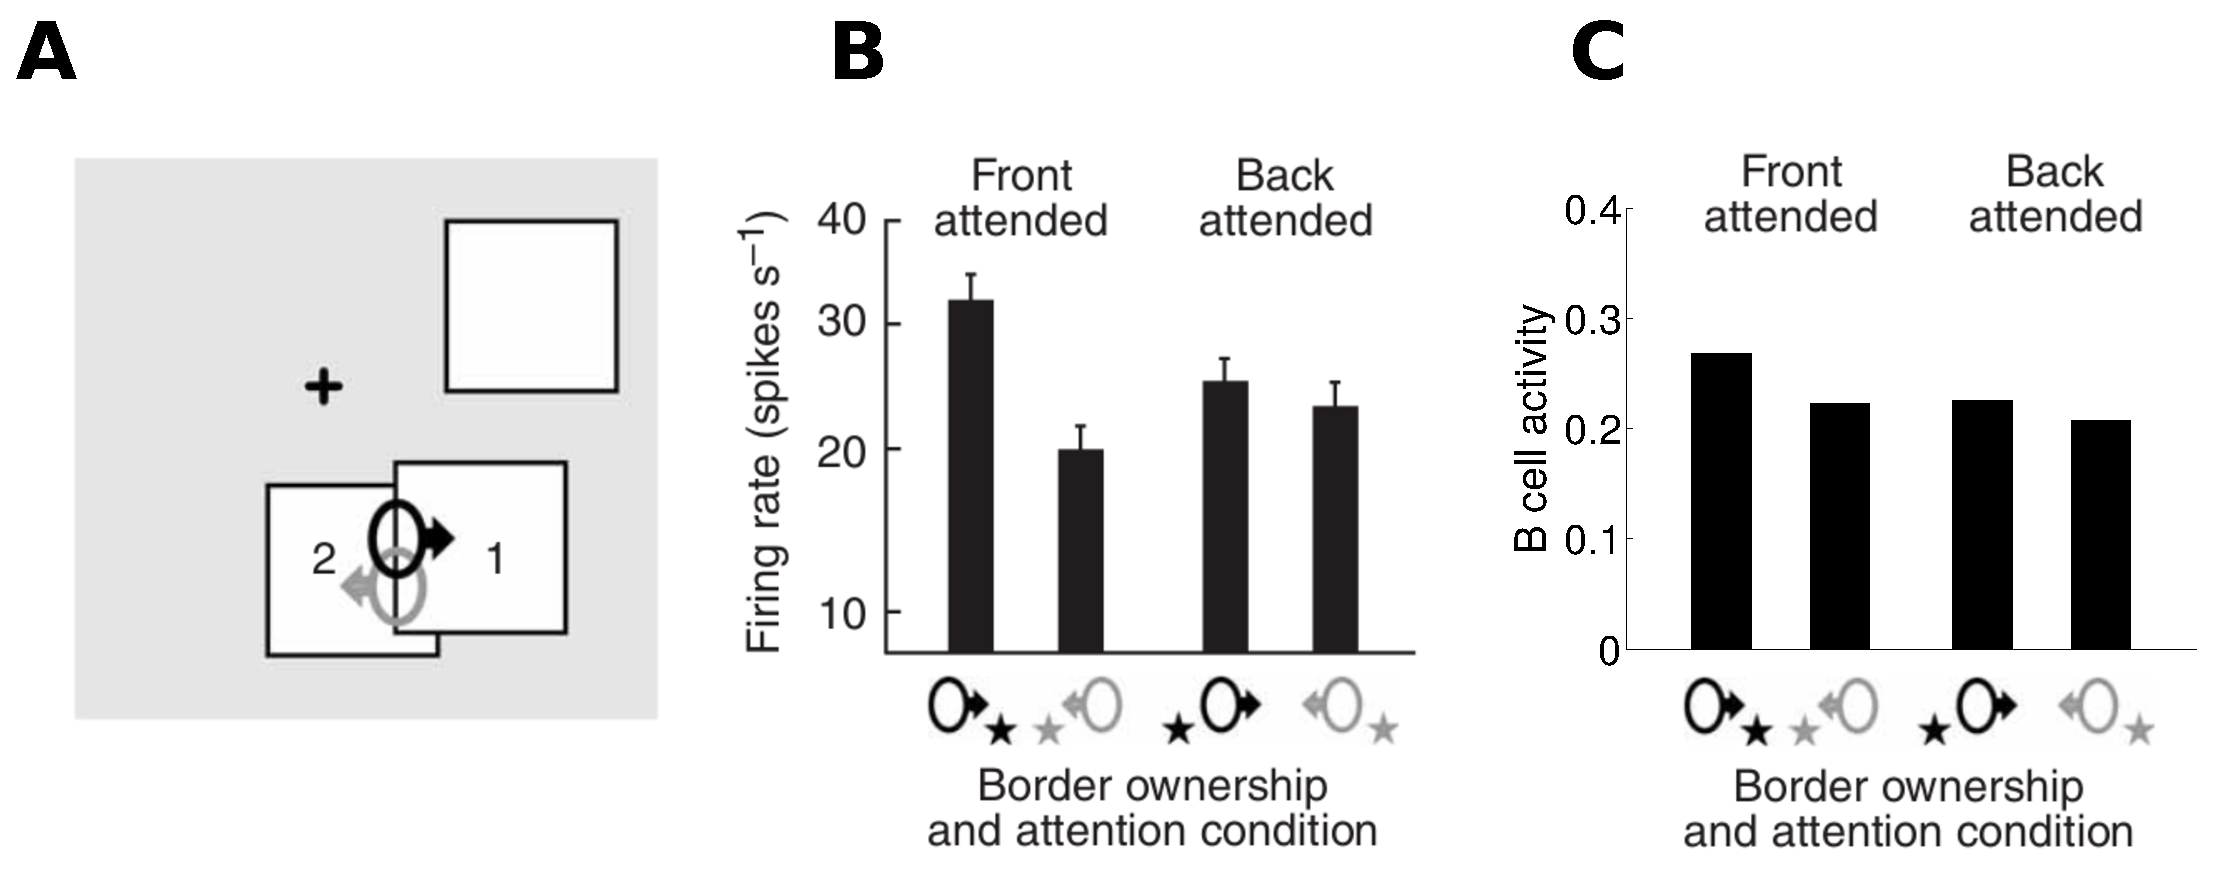
\includegraphics[width=0.75\textwidth]{Fig7.eps}
\end{center}
\caption{Quantitative comparison of model performance to
  neurophysiological findings \citep{Qiu_etal07} for border-ownership coding of
  overlapping figures. (A) The stimulus configurations used are shown,
  with neurons coding right border ownership (black) and left border
  ownership (gray) when attention was focused on either foreground
  square 1 (front attended) or on background square 2 (back
  attended). (B) The responses of border ownership selective cells
  recorded in V2 are shown:  bars indicate the
  average firing rate 
  for each stimulus condition. (C) Model B cell responses to analogous
  stimulus conditions. For both the model and the experiments,
  border-ownership modulation was strong when attention was on
  foreground but weak when attention was on background. %en
Panels~A and~B are modified from Figure~3 of~\cite{Qiu_etal07}.} 
\label{Fig:Overlap_Square_exp_model}
\end{figure*}

%bh comment here about how this lesion effectively makes our model into an alternative model?
One of the advantages of computational modeling is that it allows the
study of scenarios that are difficult to implement empirically.
One question that is difficult to answer experimentally is how removal of
feedback 
% bh be more specific
from V4 to lower visual areas
%
would change neuronal responses in V1 and V4, structures that
are known to be connected bidirectionally. This is a question that is
easily addressed in our model in what is, at the current state of
technology, a {\em Gedankenexperiment}. We eliminate all feedback from area
V4  simply by ``lesioning'' the 
connections from the grouping neurons to the V2 and V1 neurons
(setting their strength to zero), thus turning the model into a
feedforward network.  We found that this has the opposite effect of
applying attention on the $d'$ metric: the decrease in contour
response $d'$ was much larger in V1 compared to V4. Removing feedback
reduced the 7-bar contour-response $d'$ in V1 from 6.08 to 3.77, and
in V4 from 7.80 to 6.38 (Fig.~\ref{Fig:FB_att}). We note that the
contour-response $d'$ in V1 is above zero even without feedback from
grouping neurons because of the contribution of local
excitatory connections to contour integration.
This asymmetric
effect in contour response $d'$ in the two areas (V1 and V4) may point
to the different roles of feedforward and feedback processing in early
vision. We are not aware of any experimental manipulations that completely
remove feedback from area V4 without changing the circuitry in other
ways, so our results are a prediction awaiting experimental
falsification.

% bh potentially split up normal BOS results, with Qiu_etal attention results to form more distinct/clear sections
\subsection{Border ownership assignment and highlighting figures in noise}
\label{sec:BOS}
We next apply our model to understanding border ownership assignment,
discussed in Section~\ref{sec:FGO}, focusing first on the standard square
figure frequently used in neurophysiological studies of this function
\citep{Zhou_etal00,Qiu_etal07,Sugihara_etal11,Williford_vonderHeydt13,Williford_vonderHeydt14,Martin_vonderHeydt15}. Typically, the stimulus has been applied without noise. We extend
this approach by adding strong stimulus noise which was chosen as a
large number of randomly oriented bars, similar to the stimuli from
the \cite{Chen_etal14} study. In Figure~\ref{Fig:Square}, we show the
input stimulus, the edge cell activity from area V1 of our model, the
border ownership vector modulation field from V2 (defined in
Section~\ref{sec:vmi}), 
and the object and contour grouping cell
activity from V4.  Without noise (top row in the figure), our model
enhanced V1 activity along the edges of the square, correctly assigned
border ownership towards the center of the square in V2 neurons
\citep[in agreement with][] {Zhou_etal00}, and highlighted the center
of the square and the edges of the square in V4 neurons (object and
contour grouping neurons, respectively).

When noise was added to the image (bottom row of
Figure~\ref{Fig:Square}), the edges of the square, even when broken up
into different bars, were still enhanced, while the background bars
were suppressed, especially within the square.
Border ownership is still assigned correctly
along the edge of the square, but the noise results in occasional 
nonzero border ownership cell activity at other points in the image as
well. Grouping cell activity is still centered on the square, and
contour grouping neurons still highlight the edges of the squares, but
there is also noticeably increased noise.
%bh comment here about removing feedback, and that this is also an alternative model to ours?
For the square with noise, we found that attention increases the
responses of neurons along the edge of the figure (unpaired t-test,
$p=\num{2.32e-59}$) and suppresses those in the center (unpaired
t-test, $p=\num{3.42e-8}$). In addition, attention increases border
ownership modulation along the edge of the figure (unpaired t-test,
$p=\num{1.37e-143}$) and increases the activity of object grouping
neurons in the center of the figure (unpaired t-test,
$p=\num{1.53e-239}$). All effects were small but highly significant,
and were based on the differences in summed activity of neurons along
the edge or center of the figure over a total of 100 simulations.

\begin{figure*}
\begin{center}
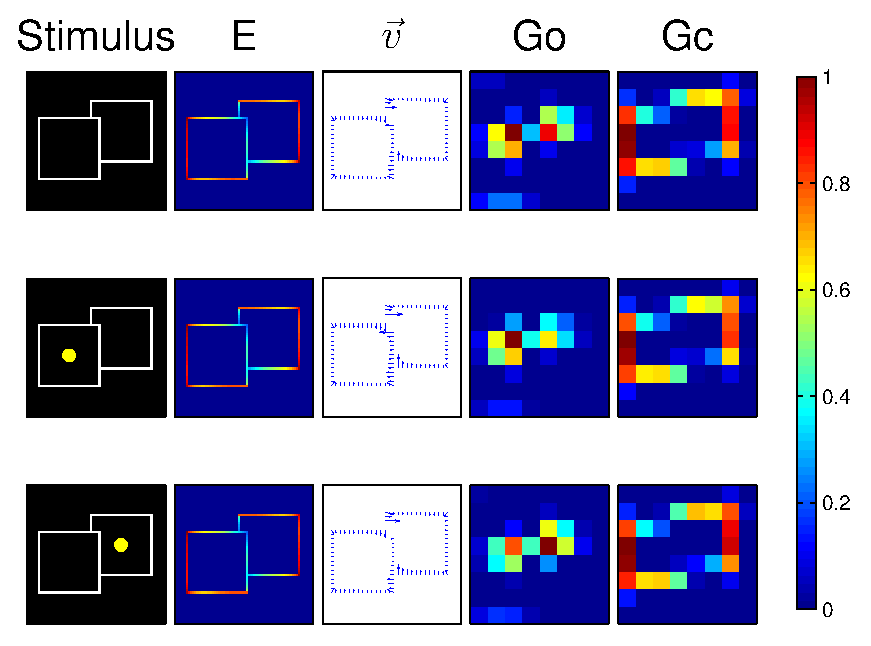
\includegraphics[width=0.75\textwidth]{Fig8.eps}
\end{center}
\caption{Attention in the presence of multiple objects. Shown are
  (left to right) the input stimulus, the edge cell activity (E), the
  border ownership assignment along edges (shown as the vector
  modulation index $\vec{v}$, section~\ref{sec:vmi}), the object
  grouping neuron activity (Go), and the contour grouping activity
  (Gc). Activities are normalized within each map, and warmer colors
  indicate higher activity (see color bar at right). The yellow dot indicates the locus of attention, which was applied at the level of grouping neurons. In
  the absence of attention (top row) or when attention is directed to
  the foreground square (middle row), the edge between the figures is
  correctly assigned to the foreground. If attention is directed
  toward the background square (bottom row), the border ownership
  signal of this edge is greatly reduced, consistent with experimental
  observations~\citep{Qiu_etal07}.}
\label{Fig:Overlap_Square}
\end{figure*}

These results demonstrate 
that the
object and contour grouping neurons  
are able to assist with
early level segmentation of a square object in noise.
Previous experimental studies have only tested squares
without noise, although the effect of figures defined by broken contours has been studied before~\citep{Zhang_vonderHeydt10}.
Our results predict that
border ownership assignment and grouping are robust even in the
presence of noise.

% bh Made this its own subsection, to more clearly separate out results
\subsection{Border ownership assignment in the presence of multiple objects}
\label{sec:BOS_overlap}
Attention must also operate in cluttered environments where multiple
objects may be present.~\cite{Qiu_etal07} studied border ownership
responses in area V2 when two overlapping squares were presented and
attention was directed either to the foreground or background square
(Figure~\ref{Fig:Overlap_Square_exp_model}A). Our model reproduces the experimental finding that  border-ownership modulation was strong when attention was on the
  foreground but weak when attention was on the background (compare Figure~\ref{Fig:Overlap_Square_exp_model}B and Figure~\ref{Fig:Overlap_Square_exp_model}C).
%bh added to clarify that there are two peaks in activity in the object grouping map, even though they are not clearly separated due to spatial proximity.
In our model, the approximate locations of the foreground and background squares are represented by two peaks in the activity of object grouping neurons (Figure~\ref{Fig:Overlap_Square}, fourth column). Selectively attending to one object enhances the activity of grouping neurons corresponding to the attended object, while simultaneously suppressing the activity of grouping neurons corresponding to the unattended object. Attentional modulation at the grouping neuron level is then propagated back to border ownership selective neurons along object boundaries via the feedback grouping circuitry of our model.
%bh Not sure why there is white space here...

 Even in the absence of attention, figure-ground segregation can be observed in the border ownership
assignment along the edges of the two squares, as well as in the
object and contour grouping cell activity
(Figure~\ref{Fig:Overlap_Square}, row 1). 
Of particular interest is
the center edge separating the foreground and background squares. When
attention is directed to the foreground square, assignment of border
ownership along this edge is strengthened
relative to the unattended case
(Figure~\ref{Fig:Overlap_Square}, row 2).
 However, if attention is
directed toward the background square, border ownership modulation of
the edge between the two squares is greatly reduced
(Figure~\ref{Fig:Overlap_Square}, row 3). 
Our results are thus in agreement
with the physiological evidence~\citep{Qiu_etal07}, and demonstrate
that grouping mechanisms provide a means to attend to objects in
clutter. 

\section{Discussion}
\label{sec:discussion}
%bh Final word count: 1413
%
Many models are tailor-made to reproduce one set of experimental results,
but from the outset we demanded
that our model explain data from two
different sets of experimental approaches, (1)~contour integration and
(2)~figure-ground segregation. 
We hypothesize that these two processes are 
 fundamentally linked in terms of the larger goal of image understanding.
Using the same set of model parameters, we reproduced several previous
experimental findings and examined the role of attention and feedback
in contour and object processing. 

\subsection{Model predictions}
Our model predicts that attentional modulation is specific to the
attended contour or object, 
rather than being defined purely
spatially. In our model, attending to the contour increased
contour-response $d'$ in both V1 and V4, consistent with experimental
results showing increased contour-related responses after animals had
been trained to perform a contour detection task, compared to when
they performed a separate set of tasks in which the contour was
behaviorally irrelevant~\citep{Li_etal08a}.  We note that
\cite{Li_etal08a} only studied neural responses in V1, while our model
makes predictions about attention-related changes to contour-response
$d'$ in both V1 and V4.

We predict that attention, in addition to enhancing the figure in an
object-based manner, may also help to suppress noise in the
background. Indeed, our model produces background suppression for
isolated contours as well as for figures embedded in noise.
Importantly, this prediction is different from what others have
observed in texture-defined figures \citep{Lamme95,Lee_etal98a}, where
there is generally response {\em enhancement} of the center of the
figure. This may be due to the nature of how the figure is defined in
our experiments -- by its contour, rather than its texture or surface.
Notably, our prediction is on a set of stimuli that has not yet been
tested experimentally (figures composed of broken contours embedded in noise).

 We also predict that removing feedback
 %bh be more explicit here about feedback, we are not talking about all cortical feedback
 from V4 to lower visual areas
 %
reduces neural responses in V1,
 while having a smaller effect in V4.
This could be tested experimentally by using the same contour
detection task used by~\cite{Chen_etal14}, and measuring the
contour-response $d'$ in V1 and V4 from reversible inactivation of
feedback connections. Although complete and selective deactivation of
% bh more specific
V4
%
feedback to areas V1 and/or V2 is technically
 challenging, there have been attempts to study the effect of 
 %bh more specific
 this type of
 %
 feedback
either through extra-striate lesions~\citep{Super_Lamme07} or
reversible inactivation~\citep{Jansen_etal12}.
Anesthesia presumably also decreases top-down influences, and indeed
reduces contour-related V1 responses \cite{Li_etal08a} and
figure-ground segregation \citep{Lamme_etal98}.

\subsection{Comparison to other models}
Many have argued that contour integration
%bh since we actually cite modeling results from both studies
 and figure-ground segregation
 %
are 
%purely
largely
%
 local phenomena
that 
%only require
rely on
%
 lateral connections
~\citep{Grossberg94, Grossberg97, Li98, Zhaoping05,
  Piech_etal13}. 
  %bh Be more fair to some models and comment that they do allow for top-down influences. Should we be more specific here? e.g. Li's feedback was to inhibitory cells, while ours is to excitatory cells and reciprocal in connections, and the mechanism of Piech's feedback is very speculative. Both models also do not have multiple visual areas, but only model processing within a single area (V1) with feedback being programmed in as a modulatory field that can somehow change parameters in V1.
  While some models have also addressed the contribution of top-down influences~\citep{Li98,Piech_etal13},
  they do not offer a clear mechanism by which higher visual areas representing object-level information can selectively feed back to lower visual areas containing feature-level information about the object.
  %
Our model is a member of a broad class of theoretical models that
achieve image understanding through bottom-up and top-down recurrent
processing~\citep{Ullman84,Hochstein_Ahissar02,Roelfsema_06,Epshtein_etal08}.
Our model is explicit in that feedback connections from higher visual areas
modulate the responses of early feature-selective neurons involved in
the related processes of contour integration and figure-ground
segregation; as such it may be a more detailed implementation of
other, more conceptual models \citep{Piech_etal13,Poort_etal12}.
One limitation of these 
latter models is that they either represent local
processing within a single area or treat each intermediate area as a
relay to higher visual areas. As a result, they cannot reproduce the
neural responses in V4 for the contour integration experiments, nor
the findings in V2 for the figure-ground segregation experiments,
where most border ownership cells are found.

\subsection{Roles of V1 and V4 in visual processing}
While V1 neurons have
small RFs that accurately code for orientation, V1 also shows strong
background inhibition off the contour. This property allows V1 neurons
to enhance contours and suppress noise in the image at a high spatial
resolution. V4 neurons, on the other hand, have large RFs that integrate
local feature information over large areas of visual space and provide
a coarse, proto-object representation of contours and objects.
Feedback from V4 can then be refined by the lateral connections present
within early visual areas, which aids in the enhancement of the figure
and its edges in the image.

%en I commented out the next paragraph to save space. It is based on
% results that we don't show so is it warranted to be in the
% length-limited Discussion session? And the effect has been mentioned
% earlier

\comment{
Our model displays stronger attention-related facilitation of neural
responses in V4 compared to V1 (results now shown), as has been
observed in many experiments~\citep[review:][]{Treue01}.  Our model
predicts that attention will increase contour-response $d'$ in V4,
while having a smaller effect in V1. One way to test this prediction
would be to perform the same contour detection task as that used
previously while controlling for the location of the focus of
attention (which was not done in the~\cite{Chen_etal14} experiments),
with the prediction that attention will improve the signal-to-noise
ratio (SNR) by effectively increasing the contour-response $d'.$ In
fact, recent results have shown that attention-related modulations in
V4 correspond closely to behavioral shifts in sensitivity or $d'$
\citep{Luo_Maunsell15}.  
}

Even when V1 neurons receive no feedback from V4 neurons,
there is an increase in contour-response $d'$ with contour
length (Figure~\ref{Fig:FB_att}). This contour facilitation is solely due to the excitatory
lateral connections present in V1, and
is weaker
without feedback. As a result, feedback
%bh more specific
from V4
%
 may not be necessary for
contour facilitation, but it interacts with local lateral connections
in a push-pull manner -- neurons along the contour are enhanced, while
elements on the background are suppressed. Not surprisingly, removing
%bh more specific
this type of
%
feedback has a larger effect on V1 neurons compared to V4 neurons,
although the activity of V4 neurons is also affected due to the
recurrency of the network model.

\subsection{Contour and object grouping neurons}
Contour grouping neurons have direct
experimental support through the recent neurophysiological experiments
published by \cite{Chen_etal14}. 
There is no clear neurophysiological evidence for object
grouping neurons yet,
although previous studies have found neurons in V4 
that respond to contour segments
of various curvatures~\citep{Pasupathy_Connor02,Brincat_Connor04}. The receptive fields of these neurons are
similar to those proposed in the model by
\cite{Craft_etal07}. Other types of grouping neurons may also exist,
including those that respond to 
gratings~\citep{Hegde_vanEssen07}, illusory
surfaces~\citep{Cox_etal13}, or 3D
surfaces~\citep{He_Nakayama95,Hu_etal15a}.
We do not attempt to model the whole array of grouping neurons that may exist, but
only those necessary for reproducing the 
neurophysiological experiments referred to here. 

In our model, orientation-independent attentional input to contour
grouping cells was used to enhance neural responses to a contour at
a given location.
We note that this form of attention is analogous to the
size- and location tolerant attentional selection process
proposed by~\cite{Mihalas_etal11b}. The
local circuitry of their model was able to sharpen a relatively broad
and nonspecific attentional input to match the size and location of a
figure in the visual scene. Similarly, the local circuitry of our
model transforms the orientation-independent attentional input such
that it only enhances the contour of the correct orientation. With
this form of attention, there is generalization over features for a
given (approximate) location.

Complementarily, feature-based attention acts broadly across the
visual scene and increases the responses of all components that share
similar feature attributes (\eg color, orientation, or direction of
movement) with the attended
component \citep{Motter94a,Treue_Trujillo99}.
Orientation-specific forms of attention
can enhance neural
responses in V1 and V4, but do not significantly alter
tuning curves or selectivity~\citep{McAdams_Maunsell99a}. 
Our model may be able to reproduce similar results by essentially changing the
form of the attentional input to be orientation-specific, \ie top-down
attention targets a \emph{single} population of contour grouping
neurons with the same orientation preference.
We expect that both
object-based and feature-based forms of attention exist and can be
flexibly used for different tasks.

\subsection{Scope and limitations of the model}
Our model seeks to reproduce two different sets of experimental
results, while making testable predictions for future experiments. 
We only included one scale of grouping neurons for
simplicity, although 
multiple scales of grouping
neurons are needed to account for the diversity in the scale of
objects in the real world.
Our model also assigns distinct roles to the
different visual areas,  edge processing in V1, border ownership
assignment in V2, and grouping of contours and objects in V4. However,
the physiological properties of neurons in early visual areas have not
been fully characterized, and 
neurons in these different
areas may have 
additional ranges of selectivity
than the ones we assign them in our model. 
Finally, our model operates on artificial
images composed of simple shapes such as contours or square
figures. In order to truly understand grouping mechanisms in natural
vision, our model must also be able to operate on natural images as
input, where the number of potential objects and features are much
richer. We are currently working  
on the construction of such a model.}
%%% Local Variables:
%%% mode: latex
%%% TeX-master: "../root"
%%% End:
